\documentclass[11pt,a4paper,titlepage]{article}
\usepackage[utf8]{inputenc}
\usepackage{amsmath,amssymb,amsthm}
\usepackage[margin=1in]{geometry}
\usepackage{hyperref}
\hypersetup{colorlinks, allcolors=blue!50!black}
% Index: the entry of a key term links to the passage that introduces the term
\makeatletter
\newcommand{\termhere}[1]{\leavevmode
  \Hy@raisedlink{\hyper@anchorstart{term:#1}\hyper@anchorend}}
\newcommand{\boxhere}[1]{\leavevmode
  \Hy@raisedlink{\hyper@anchorstart{box:#1}\hyper@anchorend}}
\makeatother
\newcommand{\termlink}[2]{\hyperlink{term:#1}{#2}}
% A key term where it is introduced: italic, with a link to its entry in the box
% of its chapter (\boxhere)
\newcommand{\keyterm}[2]{\hyperlink{box:#1}{\emph{#2}}}
\usepackage{booktabs}
\usepackage{array}
\usepackage{xcolor}
\usepackage{tikz}
\definecolor{chordblue}{HTML}{2A78D6}
\definecolor{chordorange}{HTML}{EB6834}
\usepackage{etoolbox}
\IfFileExists{imakeidx.sty}
  {\usepackage{imakeidx}\makeindex[intoc]}
  {\usepackage{makeidx}\makeindex}

% Layout: paper (default) or screen: pdflatex "\def\screenversion{}\input{file}"
\newif\ifpaper
\papertrue
\ifdefined\screenversion \paperfalse \fi

% Lean declaration and pv.py command
\newcommand{\lean}[1]{\textsf{#1}}
\newcommand{\pv}[1]{\texttt{pv.py #1}}
% number in binary
\newcommand{\bin}[1]{\text{\texttt{#1}}_2}
\ExplSyntaxOn
\seq_new:N \l__bw_parts_seq
\bool_new:N \l__bw_first_bool
\cs_new_protected:Npn \__bw_part:n #1
  {
    \fcolorbox{black!50}{black!4}
      {
        \bool_set_true:N \l__bw_first_bool
        \tl_map_inline:nn {#1}
          {
            \bool_if:NF \l__bw_first_bool { \textcolor{black!30}{\vrule width 0.3pt} }
            \bool_set_false:N \l__bw_first_bool
            \makebox[0.62em]{\rule[-0.4ex]{0pt}{2.2ex}\ttfamily ##1}
          }
      }
  }
% binary word: digits in cells, parts split at "-"
\NewDocumentCommand \bw { m }
  {
    \text
      {
        \group_begin:
        \setlength{\fboxsep}{0pt}
        \setlength{\fboxrule}{0.4pt}
        \seq_set_split:Nnn \l__bw_parts_seq { - } {#1}
        \seq_map_indexed_inline:Nn \l__bw_parts_seq
          {
            \int_compare:nNnF {##1} = {1} { \hspace{0.1em}\texttt{-}\hspace{0.1em} }
            \__bw_part:n {##2}
          }
        \group_end:
      }
  }
\ExplSyntaxOff
% Words without frames: pdflatex "\def\plainwords{}\input{file}"
\ifdefined\plainwords \RenewDocumentCommand \bw { m } {\text{\texttt{#1}}} \fi
\usepackage{listings}
\lstset{basicstyle=\ttfamily\small, columns=fullflexible, keepspaces=true}

% Glossary box at the end of each chapter
\newsavebox{\wordboxbin}
\newenvironment{wordbox}
  {\par\ifpaper\vspace*{\fill}\vspace{\bigskipamount}\else\medskip\fi
   \noindent\begin{lrbox}{\wordboxbin}%
   \begin{minipage}{\dimexpr\linewidth-2\fboxsep-2\fboxrule\relax}\small
   \textbf{Key terms introduced in Chapter~\thesection:}\par\smallskip
   \begin{tabular}{@{}>{\bfseries\boldmath}p{0.24\linewidth}p{0.68\linewidth}@{}}}
  {\end{tabular}\end{minipage}\end{lrbox}%
   \fcolorbox{black!40}{black!3}{\usebox{\wordboxbin}}\par\ifpaper\else\medskip\fi}

% A figure or table set where it stands, on one page with what follows it
\makeatletter
\newenvironment{herefloat}[1]
  {\par\addvspace{\intextsep}\noindent\begin{minipage}{\linewidth}%
   \def\@captype{#1}\centering}
  {\end{minipage}\par\nopagebreak\vspace{\intextsep}}
\makeatother

\ifpaper\pretocmd{\section}{\clearpage}{}{}\fi
\newtheorem{theorem}{Theorem}
% drop chords of 27, generated by a throwaway script
\newcommand{\dropchordsXXVII}{%
  \draw[black!45, line width=0.6pt] (0.0,0.326) -- (0.237,0.78) -- (0.475,1.229) -- (0.712,0.476) -- (0.949,0.928) -- (1.186,1.377) -- (1.424,1.822) -- (1.661,2.266) -- (1.898,2.709) -- (2.136,1.956) -- (2.373,2.4) -- (2.61,1.646) -- (2.847,2.091) -- (3.085,2.534) -- (3.322,1.781) -- (3.559,2.225) -- (3.797,2.668) -- (4.034,3.11) -- (4.271,2.357) -- (4.508,2.8) -- (4.746,3.242) -- (4.983,3.683) -- (5.22,4.124) -- (5.458,3.371) -- (5.695,3.813) -- (5.932,3.059) -- (6.169,2.306) -- (6.407,2.749) -- (6.644,3.191) -- (6.881,3.633) -- (7.119,2.879) -- (7.356,3.321) -- (7.593,3.763) -- (7.831,3.009) -- (8.068,3.451) -- (8.305,3.893) -- (8.542,4.334) -- (8.78,4.775) -- (9.017,5.215) -- (9.254,5.656) -- (9.492,4.903) -- (9.729,4.15) -- (9.966,4.591) -- (10.203,5.032) -- (10.441,5.472) -- (10.678,5.913) -- (10.915,5.16) -- (11.153,4.407) -- (11.39,3.654) -- (11.627,4.095) -- (11.864,3.342) -- (12.102,3.783) -- (12.339,3.03) -- (12.576,3.471) -- (12.814,2.718) -- (13.051,1.965) -- (13.288,1.212) -- (13.525,1.658) -- (13.763,0.905) -- (14.0,0.152);
  \draw[chordblue, line width=0.7pt] (0.0,0.326) -- (14.0,0.152);
  \draw[chordblue, line width=0.7pt] (0.237,0.78) -- (0.712,0.476);
  \draw[chordblue, line width=0.7pt] (0.712,0.476) -- (14.0,0.152);
  \draw[chordorange, dashed, line width=0.7pt] (0.949,0.928) -- (13.763,0.905);
  \draw[chordblue, line width=0.7pt] (1.186,1.377) -- (13.288,1.212);
  \draw[chordblue, line width=0.7pt] (1.424,1.822) -- (2.61,1.646);
  \draw[chordblue, line width=0.7pt] (1.661,2.266) -- (2.136,1.956);
  \draw[chordblue, line width=0.7pt] (2.136,1.956) -- (2.61,1.646);
  \draw[chordblue, line width=0.7pt] (2.61,1.646) -- (13.288,1.212);
  \draw[chordblue, line width=0.7pt] (2.847,2.091) -- (3.322,1.781);
  \draw[chordblue, line width=0.7pt] (3.322,1.781) -- (13.288,1.212);
  \draw[chordorange, dashed, line width=0.7pt] (3.559,2.225) -- (13.051,1.965);
  \draw[chordblue, line width=0.7pt] (3.797,2.668) -- (4.271,2.357);
  \draw[chordblue, line width=0.7pt] (4.271,2.357) -- (6.169,2.306);
  \draw[chordblue, line width=0.7pt] (4.508,2.8) -- (6.169,2.306);
  \draw[chordorange, dashed, line width=0.7pt] (4.746,3.242) -- (5.932,3.059);
  \draw[chordblue, line width=0.7pt] (4.983,3.683) -- (5.458,3.371);
  \draw[chordorange, dashed, line width=0.7pt] (5.458,3.371) -- (5.932,3.059);
  \draw[chordorange, dashed, line width=0.7pt] (6.169,2.306) -- (13.051,1.965);
  \draw[chordorange, dashed, line width=0.7pt] (6.407,2.749) -- (12.814,2.718);
  \draw[chordblue, line width=0.7pt] (6.644,3.191) -- (7.119,2.879);
  \draw[chordorange, dashed, line width=0.7pt] (7.119,2.879) -- (12.814,2.718);
  \draw[chordblue, line width=0.7pt] (7.356,3.321) -- (7.831,3.009);
  \draw[chordorange, dashed, line width=0.7pt] (7.831,3.009) -- (12.814,2.718);
  \draw[chordblue, line width=0.7pt] (8.068,3.451) -- (11.864,3.342);
  \draw[chordblue, line width=0.7pt] (8.305,3.893) -- (11.39,3.654);
  \draw[chordblue, line width=0.7pt] (8.542,4.334) -- (9.729,4.15);
  \draw[chordblue, line width=0.7pt] (8.78,4.775) -- (9.729,4.15);
  \draw[chordorange, dashed, line width=0.7pt] (9.017,5.215) -- (9.492,4.903);
  \draw[chordblue, line width=0.7pt] (9.729,4.15) -- (11.39,3.654);
  \draw[chordorange, dashed, line width=0.7pt] (9.966,4.591) -- (11.153,4.407);
  \draw[chordorange, dashed, line width=0.7pt] (10.203,5.032) -- (11.153,4.407);
  \draw[chordorange, dashed, line width=0.7pt] (10.441,5.472) -- (10.915,5.16);
  \draw[chordblue, line width=0.7pt] (11.39,3.654) -- (11.864,3.342);
  \draw[chordblue, line width=0.7pt] (11.864,3.342) -- (12.339,3.03);
  \draw[chordorange, dashed, line width=0.7pt] (12.339,3.03) -- (12.814,2.718);
  \draw[chordorange, dashed, line width=0.7pt] (13.288,1.212) -- (13.763,0.905);
  \fill[black!55] (0.0,0.326) circle (1.1pt);
  \fill[black!55] (0.237,0.78) circle (1.1pt);
  \fill[black!55] (0.712,0.476) circle (1.1pt);
  \fill[black!55] (0.949,0.928) circle (1.1pt);
  \fill[black!55] (1.186,1.377) circle (1.1pt);
  \fill[black!55] (1.424,1.822) circle (1.1pt);
  \fill[black!55] (1.661,2.266) circle (1.1pt);
  \fill[black!55] (2.136,1.956) circle (1.1pt);
  \fill[black!55] (2.61,1.646) circle (1.1pt);
  \fill[black!55] (2.847,2.091) circle (1.1pt);
  \fill[black!55] (3.322,1.781) circle (1.1pt);
  \fill[black!55] (3.559,2.225) circle (1.1pt);
  \fill[black!55] (3.797,2.668) circle (1.1pt);
  \fill[black!55] (4.271,2.357) circle (1.1pt);
  \fill[black!55] (4.508,2.8) circle (1.1pt);
  \fill[black!55] (4.746,3.242) circle (1.1pt);
  \fill[black!55] (4.983,3.683) circle (1.1pt);
  \fill[black!55] (5.458,3.371) circle (1.1pt);
  \fill[black!55] (6.169,2.306) circle (1.1pt);
  \fill[black!55] (6.407,2.749) circle (1.1pt);
  \fill[black!55] (6.644,3.191) circle (1.1pt);
  \fill[black!55] (7.119,2.879) circle (1.1pt);
  \fill[black!55] (7.356,3.321) circle (1.1pt);
  \fill[black!55] (7.831,3.009) circle (1.1pt);
  \fill[black!55] (8.068,3.451) circle (1.1pt);
  \fill[black!55] (8.305,3.893) circle (1.1pt);
  \fill[black!55] (8.542,4.334) circle (1.1pt);
  \fill[black!55] (8.78,4.775) circle (1.1pt);
  \fill[black!55] (9.017,5.215) circle (1.1pt);
  \fill[black!55] (9.729,4.15) circle (1.1pt);
  \fill[black!55] (9.966,4.591) circle (1.1pt);
  \fill[black!55] (10.203,5.032) circle (1.1pt);
  \fill[black!55] (10.441,5.472) circle (1.1pt);
  \fill[black!55] (11.39,3.654) circle (1.1pt);
  \fill[black!55] (11.864,3.342) circle (1.1pt);
  \fill[black!55] (12.339,3.03) circle (1.1pt);
  \fill[black!55] (13.288,1.212) circle (1.1pt);
}
\newcommand{\dropchordsXXVIIlabels}{%
  \node[left, font=\small] at (0.0,0.326) {$27$};
  \node[right, font=\small] at (14.0,0.152) {$23$};
  \node[above, font=\small] at (10.678,5.913) {$4\,616$};
  \draw[black!40] (0,-0.25) -- (14.0,-0.25);
  \node[below, font=\small] at (0,-0.25) {step $0$};
  \node[below, font=\small] at (14.0,-0.25) {step $59$};
}
% counting grid, generated by a throwaway script
\newcommand{\countgrid}{%
  \draw[black!35] (0.00,0.00) -- (1.05,0.00);
  \draw[black!35] (0.00,0.00) -- (0.00,-0.80);
  \draw[black!35] (1.05,0.00) -- (2.10,0.00);
  \draw[black!35] (1.05,0.00) -- (1.05,-0.80);
  \draw[black!35] (2.10,0.00) -- (3.15,0.00);
  \draw[black!35] (2.10,0.00) -- (2.10,-0.80);
  \draw[black!35] (2.10,-0.80) -- (3.15,-0.80);
  \draw[black!35] (2.10,-0.80) -- (2.10,-1.60);
  \draw[black!35] (3.15,0.00) -- (4.20,0.00);
  \draw[black!35] (3.15,0.00) -- (3.15,-0.80);
  \draw[black!35] (3.15,-0.80) -- (4.20,-0.80);
  \draw[black!35] (3.15,-0.80) -- (3.15,-1.60);
  \draw[black!35] (4.20,0.00) -- (5.25,0.00);
  \draw[black!35] (4.20,0.00) -- (4.20,-0.80);
  \draw[black!35] (4.20,-0.80) -- (5.25,-0.80);
  \draw[black!35] (4.20,-0.80) -- (4.20,-1.60);
  \draw[black!35] (5.25,0.00) -- (6.30,0.00);
  \draw[black!35] (5.25,0.00) -- (5.25,-0.80);
  \draw[black!35] (4.20,-1.60) -- (5.25,-1.60);
  \draw[black!35] (4.20,-1.60) -- (4.20,-2.40);
  \draw[black!35] (5.25,-0.80) -- (6.30,-0.80);
  \draw[black!35] (5.25,-0.80) -- (5.25,-1.60);
  \draw[black!35] (6.30,0.00) -- (6.30,-0.80);
  \draw[black!35] (5.25,-1.60) -- (6.30,-1.60);
  \draw[black!35] (5.25,-1.60) -- (5.25,-2.40);
  \draw[black!35] (6.30,-0.80) -- (6.30,-1.60);
  \draw[black!35] (6.30,-1.60) -- (6.30,-2.40);
  \draw[black!35] (6.30,-2.40) -- (6.30,-3.20);
  \node[circle, fill=white, draw=black!40, inner sep=1.5pt, font=\small] at (0.00,0.00) {$1$};
  \node[circle, fill=chordblue!35, draw=chordblue, inner sep=1.5pt, font=\small\bfseries] at (0.00,-0.80) {$1$};
  \node[circle, fill=white, draw=black!40, inner sep=1.5pt, font=\small] at (1.05,0.00) {$1$};
  \node[circle, fill=chordblue!35, draw=chordblue, inner sep=1.5pt, font=\small\bfseries] at (1.05,-0.80) {$1$};
  \node[circle, fill=white, draw=black!40, inner sep=1.5pt, font=\small] at (2.10,0.00) {$1$};
  \node[circle, fill=white, draw=black!40, inner sep=1.5pt, font=\small] at (2.10,-0.80) {$1$};
  \node[circle, fill=chordblue!35, draw=chordblue, inner sep=1.5pt, font=\small\bfseries] at (2.10,-1.60) {$1$};
  \node[circle, fill=white, draw=black!40, inner sep=1.5pt, font=\small] at (3.15,0.00) {$1$};
  \node[circle, fill=white, draw=black!40, inner sep=1.5pt, font=\small] at (3.15,-0.80) {$2$};
  \node[circle, fill=chordblue!35, draw=chordblue, inner sep=1.5pt, font=\small\bfseries] at (3.15,-1.60) {$2$};
  \node[circle, fill=white, draw=black!40, inner sep=1.5pt, font=\small] at (4.20,0.00) {$1$};
  \node[circle, fill=white, draw=black!40, inner sep=1.5pt, font=\small] at (4.20,-0.80) {$3$};
  \node[circle, fill=white, draw=black!40, inner sep=1.5pt, font=\small] at (4.20,-1.60) {$3$};
  \node[circle, fill=chordblue!35, draw=chordblue, inner sep=1.5pt, font=\small\bfseries] at (4.20,-2.40) {$3$};
  \node[circle, fill=white, draw=black!40, inner sep=1.5pt, font=\small] at (5.25,0.00) {$1$};
  \node[circle, fill=white, draw=black!40, inner sep=1.5pt, font=\small] at (5.25,-0.80) {$4$};
  \node[circle, fill=white, draw=black!40, inner sep=1.5pt, font=\small] at (5.25,-1.60) {$7$};
  \node[circle, fill=chordblue!35, draw=chordblue, inner sep=1.5pt, font=\small\bfseries] at (5.25,-2.40) {$7$};
  \node[circle, fill=white, draw=black!40, inner sep=1.5pt, font=\small] at (6.30,0.00) {$1$};
  \node[circle, fill=white, draw=black!40, inner sep=1.5pt, font=\small] at (6.30,-0.80) {$5$};
  \node[circle, fill=white, draw=black!40, inner sep=1.5pt, font=\small] at (6.30,-1.60) {$12$};
  \node[circle, fill=white, draw=black!40, inner sep=1.5pt, font=\small] at (6.30,-2.40) {$12$};
  \node[circle, fill=chordblue!35, draw=chordblue, inner sep=1.5pt, font=\small\bfseries] at (6.30,-3.20) {$12$};
  \node[font=\small, anchor=west] at (-0.3,1.0) {\bw{1}: one step right};
  \node[font=\small, anchor=west] at (-0.3,0.6) {\bw{0}: one step down};
}
% building with stairs and poles, generated by a throwaway script
\newcommand{\stairsbuilding}{%
  \draw[black!50, fill=black!3] (0,0.19) rectangle (3.00,7.79);
  \draw[black!25] (0,0.57) -- (3.00,0.57);
  \draw[black!25] (0,0.95) -- (3.00,0.95);
  \draw[black!25] (0,1.33) -- (3.00,1.33);
  \draw[black!25] (0,1.71) -- (3.00,1.71);
  \draw[black!25] (0,2.09) -- (3.00,2.09);
  \draw[black!25] (0,2.47) -- (3.00,2.47);
  \draw[black!25] (0,2.85) -- (3.00,2.85);
  \draw[black!25] (0,3.23) -- (3.00,3.23);
  \draw[black!25] (0,3.61) -- (3.00,3.61);
  \draw[black!25] (0,3.99) -- (3.00,3.99);
  \draw[black!25] (0,4.37) -- (3.00,4.37);
  \draw[black!25] (0,4.75) -- (3.00,4.75);
  \draw[black!25] (0,5.13) -- (3.00,5.13);
  \draw[black!25] (0,5.51) -- (3.00,5.51);
  \draw[black!25] (0,5.89) -- (3.00,5.89);
  \draw[black!25] (0,6.27) -- (3.00,6.27);
  \draw[black!25] (0,6.65) -- (3.00,6.65);
  \draw[black!25] (0,7.03) -- (3.00,7.03);
  \draw[black!25] (0,7.41) -- (3.00,7.41);
  \node[font=\scriptsize, anchor=west] at (0.05,0.38) {$1$};
  \node[font=\scriptsize, anchor=west] at (0.05,0.76) {$2$};
  \node[font=\scriptsize, anchor=west] at (0.05,1.14) {$3$};
  \node[font=\scriptsize, anchor=west] at (0.05,1.52) {$4$};
  \node[font=\scriptsize, anchor=west] at (0.05,1.90) {$5$};
  \node[font=\scriptsize, anchor=west] at (0.05,2.28) {$6$};
  \node[font=\scriptsize, anchor=west] at (0.05,2.66) {$7$};
  \node[font=\scriptsize, anchor=west] at (0.05,3.04) {$8$};
  \node[font=\scriptsize, anchor=west] at (0.05,3.42) {$9$};
  \node[font=\scriptsize, anchor=west] at (0.05,3.80) {$10$};
  \node[font=\scriptsize, anchor=west] at (0.05,4.18) {$11$};
  \node[font=\scriptsize, anchor=west] at (0.05,4.56) {$12$};
  \node[font=\scriptsize, anchor=west] at (0.05,4.94) {$13$};
  \node[font=\scriptsize, anchor=west] at (0.05,5.32) {$14$};
  \node[font=\scriptsize, anchor=west] at (0.05,5.70) {$15$};
  \node[font=\scriptsize, anchor=west] at (0.05,6.08) {$16$};
  \node[font=\scriptsize, anchor=west] at (0.05,6.46) {$17$};
  \node[font=\scriptsize, anchor=west] at (0.05,6.84) {$18$};
  \node[font=\scriptsize, anchor=west] at (0.05,7.22) {$19$};
  \node[font=\scriptsize, anchor=west] at (0.05,7.60) {$20$};
  \draw[black!3, line width=3pt] (0.77,0.57) -- (0.77,0.57);
  \draw[black!45, line width=0.3pt, fill=white] (0.71,0.38) rectangle (0.83,0.76);
  \draw[chordorange, line width=1pt] (0.77,0.76) -- (0.77,0.38);
  \fill[chordorange] (0.77,0.76) circle (1.3pt);
  \node[font=\scriptsize, anchor=east, inner sep=1pt] at (0.77,0.76) {\bw{0}};
  \draw[chordorange, -stealth, line width=0.5pt] (0.77,0.38) -- (0.89,0.38);
  \draw[black!3, line width=3pt] (0.99,1.33) -- (0.99,0.95);
  \draw[black!45, line width=0.3pt, fill=white] (0.93,0.76) rectangle (1.05,1.52);
  \draw[chordorange, line width=1pt] (0.99,1.52) -- (0.99,0.76);
  \fill[chordorange] (0.99,1.52) circle (1.3pt);
  \node[font=\scriptsize, anchor=east, inner sep=1pt] at (0.99,1.52) {\bw{0}};
  \draw[chordorange, -stealth, line width=0.5pt] (0.99,0.76) -- (1.11,0.76);
  \draw[black!3, line width=3pt] (1.21,2.09) -- (1.21,1.33);
  \draw[black!45, line width=0.3pt, fill=white] (1.15,1.14) rectangle (1.27,2.28);
  \draw[chordorange, line width=1pt] (1.21,2.28) -- (1.21,1.14);
  \fill[chordorange] (1.21,2.28) circle (1.3pt);
  \node[font=\scriptsize, anchor=east, inner sep=1pt] at (1.21,2.28) {\bw{0}};
  \draw[chordorange, -stealth, line width=0.5pt] (1.21,1.14) -- (1.33,1.14);
  \draw[black!3, line width=3pt] (1.43,2.85) -- (1.43,1.71);
  \draw[black!45, line width=0.3pt, fill=white] (1.37,1.52) rectangle (1.49,3.04);
  \draw[chordorange, line width=1pt] (1.43,3.04) -- (1.43,1.52);
  \fill[chordorange] (1.43,3.04) circle (1.3pt);
  \node[font=\scriptsize, anchor=east, inner sep=1pt] at (1.43,3.04) {\bw{0}};
  \draw[chordorange, -stealth, line width=0.5pt] (1.43,1.52) -- (1.55,1.52);
  \draw[black!3, line width=3pt] (1.65,3.61) -- (1.65,2.09);
  \draw[black!45, line width=0.3pt, fill=white] (1.59,1.90) rectangle (1.71,3.80);
  \draw[chordorange, line width=1pt] (1.65,3.80) -- (1.65,1.90);
  \fill[chordorange] (1.65,3.80) circle (1.3pt);
  \node[font=\scriptsize, anchor=east, inner sep=1pt] at (1.65,3.80) {\bw{0}};
  \draw[chordorange, -stealth, line width=0.5pt] (1.65,1.90) -- (1.77,1.90);
  \draw[black!3, line width=3pt] (1.87,4.37) -- (1.87,2.47);
  \draw[black!45, line width=0.3pt, fill=white] (1.81,2.28) rectangle (1.93,4.56);
  \draw[chordorange, line width=1pt] (1.87,4.56) -- (1.87,2.28);
  \fill[chordorange] (1.87,4.56) circle (1.3pt);
  \node[font=\scriptsize, anchor=east, inner sep=1pt] at (1.87,4.56) {\bw{0}};
  \draw[chordorange, -stealth, line width=0.5pt] (1.87,2.28) -- (1.99,2.28);
  \draw[black!3, line width=3pt] (2.09,5.13) -- (2.09,2.85);
  \draw[black!45, line width=0.3pt, fill=white] (2.03,2.66) rectangle (2.15,5.32);
  \draw[chordorange, line width=1pt] (2.09,5.32) -- (2.09,2.66);
  \fill[chordorange] (2.09,5.32) circle (1.3pt);
  \node[font=\scriptsize, anchor=east, inner sep=1pt] at (2.09,5.32) {\bw{0}};
  \draw[chordorange, -stealth, line width=0.5pt] (2.09,2.66) -- (2.21,2.66);
  \draw[black!3, line width=3pt] (2.31,5.89) -- (2.31,3.23);
  \draw[black!45, line width=0.3pt, fill=white] (2.25,3.04) rectangle (2.37,6.08);
  \draw[chordorange, line width=1pt] (2.31,6.08) -- (2.31,3.04);
  \fill[chordorange] (2.31,6.08) circle (1.3pt);
  \node[font=\scriptsize, anchor=east, inner sep=1pt] at (2.31,6.08) {\bw{0}};
  \draw[chordorange, -stealth, line width=0.5pt] (2.31,3.04) -- (2.43,3.04);
  \draw[black!3, line width=3pt] (2.53,6.65) -- (2.53,3.61);
  \draw[black!45, line width=0.3pt, fill=white] (2.47,3.42) rectangle (2.59,6.84);
  \draw[chordorange, line width=1pt] (2.53,6.84) -- (2.53,3.42);
  \fill[chordorange] (2.53,6.84) circle (1.3pt);
  \node[font=\scriptsize, anchor=east, inner sep=1pt] at (2.53,6.84) {\bw{0}};
  \draw[chordorange, -stealth, line width=0.5pt] (2.53,3.42) -- (2.65,3.42);
  \draw[black!3, line width=3pt] (2.75,7.41) -- (2.75,3.99);
  \draw[black!45, line width=0.3pt, fill=white] (2.69,3.80) rectangle (2.81,7.60);
  \draw[chordorange, line width=1pt] (2.75,7.60) -- (2.75,3.80);
  \fill[chordorange] (2.75,7.60) circle (1.3pt);
  \node[font=\scriptsize, anchor=east, inner sep=1pt] at (2.75,7.60) {\bw{0}};
  \draw[chordorange, -stealth, line width=0.5pt] (2.75,3.80) -- (2.87,3.80);
  \draw[chordblue, -stealth, line width=0.5pt] (0,0.38) to[out=180, in=180, looseness=0.9] node[pos=0, anchor=south east, xshift=-1pt, yshift=1pt, font=\scriptsize, inner sep=0pt, text=black] {\bw{1}} (0,0.76);
  \draw[chordblue, -stealth, line width=0.5pt] (0,1.14) to[out=180, in=180, looseness=0.9] node[pos=0, anchor=south east, xshift=-1pt, yshift=1pt, font=\scriptsize, inner sep=0pt, text=black] {\bw{1}} (0,1.90);
  \draw[chordblue, -stealth, line width=0.5pt] (0,1.90) to[out=180, in=180, looseness=0.9] node[pos=0, anchor=south east, xshift=-1pt, yshift=1pt, font=\scriptsize, inner sep=0pt, text=black] {\bw{1}} (0,3.04);
  \draw[chordblue, -stealth, line width=0.5pt] (0,2.66) to[out=180, in=180, looseness=0.9] node[pos=0, anchor=south east, xshift=-1pt, yshift=1pt, font=\scriptsize, inner sep=0pt, text=black] {\bw{1}} (0,4.18);
  \draw[chordblue, -stealth, line width=0.5pt] (0,3.42) to[out=180, in=180, looseness=0.9] node[pos=0, anchor=south east, xshift=-1pt, yshift=1pt, font=\scriptsize, inner sep=0pt, text=black] {\bw{1}} (0,5.32);
  \draw[chordblue, -stealth, line width=0.5pt] (0,4.18) to[out=180, in=180, looseness=0.9] node[pos=0, anchor=south east, xshift=-1pt, yshift=1pt, font=\scriptsize, inner sep=0pt, text=black] {\bw{1}} (0,6.46);
  \draw[chordblue, -stealth, line width=0.5pt] (0,4.94) to[out=180, in=180, looseness=0.9] node[pos=0, anchor=south east, xshift=-1pt, yshift=1pt, font=\scriptsize, inner sep=0pt, text=black] {\bw{1}} (0,7.60);
  \draw[chordblue, -stealth, line width=0.5pt] (0,5.70) -- (-1.45,8.40) node[pos=0, anchor=south east, xshift=-1pt, yshift=1pt, font=\scriptsize, inner sep=0pt, text=black] {\bw{1}} node[above, font=\tiny, text=chordblue] {$23$};
  \draw[chordblue, -stealth, line width=0.5pt] (0,6.46) -- (-1.69,8.58) node[pos=0, anchor=south east, xshift=-1pt, yshift=1pt, font=\scriptsize, inner sep=0pt, text=black] {\bw{1}} node[above, font=\tiny, text=chordblue] {$26$};
  \draw[chordblue, -stealth, line width=0.5pt] (0,7.22) -- (-1.93,8.76) node[pos=0, anchor=south east, xshift=-1pt, yshift=1pt, font=\scriptsize, inner sep=0pt, text=black] {\bw{1}} node[above, font=\tiny, text=chordblue] {$29$};
}
% sub-drops of 123, generated by a throwaway script
\newcommand{\subdropsCXXIII}{%
  \node[font=\small] at (0.00,0) {$123$};
  \node[font=\small] at (1.25,0) {$185$};
  \node[font=\small] at (1.875,-0.02) {,};
  \node[font=\small] at (2.50,0) {$278$};
  \node[font=\small] at (3.125,-0.02) {,};
  \node[font=\small] at (3.75,0) {$139$};
  \node[font=\small] at (4.375,-0.02) {,};
  \node[font=\small] at (5.00,0) {$209$};
  \node[font=\small] at (5.625,-0.02) {,};
  \node[font=\small] at (6.25,0) {$314$};
  \node[font=\small] at (6.875,-0.02) {,};
  \node[font=\small] at (7.50,0) {$157$};
  \node[font=\small] at (8.125,-0.02) {,};
  \node[font=\small] at (8.75,0) {$236$};
  \node[font=\small] at (9.375,-0.02) {,};
  \node[font=\small] at (10.00,0) {$118$};
  \node[font=\small] at (0.562,0) {:};
  \draw[chordblue, line width=1.6pt] (-0.30,-0.42) -- (10.30,-0.42);
  \draw[chordblue, line width=0.8pt] (10.30,-0.27) -- (10.30,-0.57);
  \draw[chordblue, line width=1.6pt] (0.95,-0.84) -- (4.05,-0.84);
  \draw[chordblue, line width=0.8pt] (4.05,-0.69) -- (4.05,-0.99);
  \draw[black!40, line width=1.6pt] (2.20,-1.26) -- (4.05,-1.26);
  \draw[black!40, line width=0.8pt] (4.05,-1.11) -- (4.05,-1.41);
  \draw[chordblue, line width=1.6pt] (3.45,-1.68) -- (10.30,-1.68);
  \draw[chordblue, line width=0.8pt] (10.30,-1.53) -- (10.30,-1.83);
  \draw[chordblue, line width=1.6pt] (4.70,-2.10) -- (7.80,-2.10);
  \draw[chordblue, line width=0.8pt] (7.80,-1.95) -- (7.80,-2.25);
  \draw[black!40, line width=1.6pt] (5.95,-2.52) -- (7.80,-2.52);
  \draw[black!40, line width=0.8pt] (7.80,-2.37) -- (7.80,-2.67);
  \draw[chordblue, line width=1.6pt] (7.20,-2.94) -- (10.30,-2.94);
  \draw[chordblue, line width=0.8pt] (10.30,-2.79) -- (10.30,-3.09);
  \draw[black!40, line width=1.6pt] (8.45,-3.36) -- (10.30,-3.36);
  \draw[black!40, line width=0.8pt] (10.30,-3.21) -- (10.30,-3.51);
}
% mountain of 123, generated by a throwaway script
\newcommand{\mountainCXXIII}{%
  \draw[black!30] (0,0) -- (7.50,0);
  \draw[chordblue, line width=1.2pt] (0.00,0.00) -- (0.75,0.60);
  \node[font=\scriptsize, above left, text=chordblue] at (0.38,0.30) {$123$};
  \draw[chordblue, line width=1.2pt] (0.75,0.60) -- (1.50,1.20);
  \node[font=\scriptsize, above left, text=chordblue] at (1.12,0.90) {$185$};
  \draw[chordorange, line width=1.2pt] (1.50,1.20) -- (2.25,0.60);
  \node[font=\scriptsize, below left, text=chordorange] at (1.88,0.90) {$139$};
  \draw[chordblue, line width=1.2pt] (2.25,0.60) -- (3.00,1.20);
  \node[font=\scriptsize, above left, text=chordblue] at (2.62,0.90) {$139$};
  \draw[chordblue, line width=1.2pt] (3.00,1.20) -- (3.75,1.80);
  \node[font=\scriptsize, above left, text=chordblue] at (3.38,1.50) {$209$};
  \draw[chordorange, line width=1.2pt] (3.75,1.80) -- (4.50,1.20);
  \node[font=\scriptsize, below left, text=chordorange] at (4.12,1.50) {$157$};
  \draw[chordblue, line width=1.2pt] (4.50,1.20) -- (5.25,1.80);
  \node[font=\scriptsize, above left, text=chordblue] at (4.88,1.50) {$157$};
  \draw[chordorange, line width=1.2pt] (5.25,1.80) -- (6.00,1.20);
  \node[font=\scriptsize, below left, text=chordorange] at (5.62,1.50) {$118$};
  \draw[chordorange, line width=1.2pt] (6.00,1.20) -- (6.75,0.60);
  \node[font=\scriptsize, below left, text=chordorange] at (6.38,0.90) {$118$};
  \draw[chordorange, line width=1.2pt] (6.75,0.60) -- (7.50,0.00);
  \node[font=\scriptsize, below left, text=chordorange] at (6.95,0.44) {$118$};
}
% comic page of the young engineer, generated by a throwaway script
\newcommand{\comicengineer}{%
  \begin{scope}[shift={(0.00,6.40)}]
    \draw[black!70, line width=0.8pt] (0,0) rectangle (7,6);
    \node[font=\small\bfseries, anchor=north west, text width=6.6cm] at (0.1,5.95) {1. Every floor has one way out: a stair up or a pole down.};
    \draw[black!50, fill=black!3] (2.20,0.50) rectangle (3.80,4.90);
    \draw[black!25] (2.20,1.05) -- (3.80,1.05);
    \draw[black!25] (2.20,1.60) -- (3.80,1.60);
    \draw[black!25] (2.20,2.15) -- (3.80,2.15);
    \draw[black!25] (2.20,2.70) -- (3.80,2.70);
    \draw[black!25] (2.20,3.25) -- (3.80,3.25);
    \draw[black!25] (2.20,3.80) -- (3.80,3.80);
    \draw[black!25] (2.20,4.35) -- (3.80,4.35);
    \node[font=\tiny, anchor=east] at (2.15,0.68) {1};
    \node[font=\tiny, anchor=east] at (2.15,1.23) {2};
    \node[font=\tiny, anchor=east] at (2.15,1.77) {3};
    \node[font=\tiny, anchor=east] at (2.15,2.33) {4};
    \node[font=\tiny, anchor=east] at (2.15,2.88) {5};
    \node[font=\tiny, anchor=east] at (2.15,3.43) {6};
    \node[font=\tiny, anchor=east] at (2.15,3.98) {7};
    \node[font=\tiny, anchor=east] at (2.15,4.53) {8};
    \draw[chordblue, -stealth, line width=0.7pt] (2.20,1.68) to[out=180, in=180, looseness=1.2] node[midway, left, font=\tiny, text=chordblue] {1} (2.20,2.77);
    \draw[chordblue, -stealth, line width=0.7pt] (2.20,2.77) to[out=180, in=180, looseness=1.2] node[midway, left, font=\tiny, text=chordblue] {1} (2.20,4.42);
    \draw[chordblue, -stealth, line width=0.7pt] (2.20,0.57) to[out=180, in=180, looseness=1.2] node[midway, left, font=\tiny, text=chordblue] {1} (2.20,1.13);
    \draw[chordorange, line width=1.1pt] (2.75,1.08) -- (2.75,0.53);
    \draw[chordorange, line width=1.1pt] (3.00,2.18) -- (3.00,1.08);
    \draw[chordorange, line width=1.1pt] (3.25,3.28) -- (3.25,1.62);
    \draw[chordorange, line width=1.1pt] (3.50,4.38) -- (3.50,2.18);
    \begin{scope}[shift={(4.15,1.60)}, black, line width=0.7pt]
      \draw (0,0.36) circle (0.07);
      \draw (0,0.29) -- (0,0.13);
      \draw (0,0.13) -- (-0.07,0);
      \draw (0,0.13) -- (0.07,0);
      \draw (-0.09,0.23) -- (0.09,0.23);
    \end{scope}
  \end{scope}
  \begin{scope}[shift={(7.40,6.40)}]
    \draw[black!70, line width=0.8pt] (0,0) rectangle (7,6);
    \node[font=\small\bfseries, anchor=north west, text width=6.6cm] at (0.1,5.95) {2. A very young engineer has an idea.};
    \draw[black!50, fill=black!3] (2.20,0.50) rectangle (3.80,4.90);
    \draw[black!25] (2.20,1.05) -- (3.80,1.05);
    \draw[black!25] (2.20,1.60) -- (3.80,1.60);
    \draw[black!25] (2.20,2.15) -- (3.80,2.15);
    \draw[black!25] (2.20,2.70) -- (3.80,2.70);
    \draw[black!25] (2.20,3.25) -- (3.80,3.25);
    \draw[black!25] (2.20,3.80) -- (3.80,3.80);
    \draw[black!25] (2.20,4.35) -- (3.80,4.35);
    \node[font=\tiny, anchor=east] at (2.15,0.68) {1};
    \node[font=\tiny, anchor=east] at (2.15,1.23) {2};
    \node[font=\tiny, anchor=east] at (2.15,1.77) {3};
    \node[font=\tiny, anchor=east] at (2.15,2.33) {4};
    \node[font=\tiny, anchor=east] at (2.15,2.88) {5};
    \node[font=\tiny, anchor=east] at (2.15,3.43) {6};
    \node[font=\tiny, anchor=east] at (2.15,3.98) {7};
    \node[font=\tiny, anchor=east] at (2.15,4.53) {8};
    \draw[chordblue, -stealth, line width=0.7pt] (2.20,1.68) to[out=180, in=180, looseness=1.2] node[midway, left, font=\tiny, text=chordblue] {1} (2.20,2.77);
    \draw[chordblue, -stealth, line width=0.7pt] (2.20,2.77) to[out=180, in=180, looseness=1.2] node[midway, left, font=\tiny, text=chordblue] {1} (2.20,4.42);
    \draw[chordorange, line width=1.1pt, dashed] (3.50,4.38) -- (3.50,0.53);
    \begin{scope}[shift={(5.40,0.50)}, black, line width=0.7pt]
      \draw (0,0.36) circle (0.07);
      \draw (0,0.29) -- (0,0.13);
      \draw (0,0.13) -- (-0.07,0);
      \draw (0,0.13) -- (0.07,0);
      \draw (-0.09,0.23) -- (0.09,0.23);
      \fill[chordorange] (-0.09,0.40) arc (180:0:0.09) -- cycle;
    \end{scope}
    \node[draw=black!60, fill=white, rounded corners=3pt, font=\scriptsize, text width=2.6cm, align=center] (b) at (5.30,3.20) {Why stop halfway? Everybody goes all the way down to 1. One long pole does it!};
    \draw[black!60] (b.south) -- (5.40,1.00);
  \end{scope}
  \begin{scope}[shift={(0.00,0.00)}]
    \draw[black!70, line width=0.8pt] (0,0) rectangle (7,6);
    \node[font=\small\bfseries, anchor=north west, text width=6.6cm] at (0.1,5.95) {3. The first ride.};
    \draw[black!50, fill=black!3] (2.20,0.50) rectangle (3.80,4.90);
    \draw[black!25] (2.20,1.05) -- (3.80,1.05);
    \draw[black!25] (2.20,1.60) -- (3.80,1.60);
    \draw[black!25] (2.20,2.15) -- (3.80,2.15);
    \draw[black!25] (2.20,2.70) -- (3.80,2.70);
    \draw[black!25] (2.20,3.25) -- (3.80,3.25);
    \draw[black!25] (2.20,3.80) -- (3.80,3.80);
    \draw[black!25] (2.20,4.35) -- (3.80,4.35);
    \node[font=\tiny, anchor=east] at (2.15,0.68) {1};
    \node[font=\tiny, anchor=east] at (2.15,1.23) {2};
    \node[font=\tiny, anchor=east] at (2.15,1.77) {3};
    \node[font=\tiny, anchor=east] at (2.15,2.33) {4};
    \node[font=\tiny, anchor=east] at (2.15,2.88) {5};
    \node[font=\tiny, anchor=east] at (2.15,3.43) {6};
    \node[font=\tiny, anchor=east] at (2.15,3.98) {7};
    \node[font=\tiny, anchor=east] at (2.15,4.53) {8};
    \draw[chordblue, -stealth, line width=0.7pt] (2.20,1.68) to[out=180, in=180, looseness=1.2] node[midway, left, font=\tiny, text=chordblue] {1} (2.20,2.77);
    \draw[chordblue, -stealth, line width=0.7pt] (2.20,2.77) to[out=180, in=180, looseness=1.2] node[midway, left, font=\tiny, text=chordblue] {1} (2.20,4.42);
    \draw[chordorange, line width=1.1pt] (3.50,4.38) -- (3.50,0.53);
    \begin{scope}[shift={(3.50,2.77)}, chordblue, line width=0.7pt]
      \draw (0,0.36) circle (0.07);
      \draw (0,0.29) -- (0,0.13);
      \draw (0,0.13) -- (-0.07,0);
      \draw (0,0.13) -- (0.07,0);
      \draw (-0.09,0.23) -- (0.09,0.23);
    \end{scope}
    \draw[chordblue, -stealth, line width=0.6pt] (3.75,3.53) -- (3.75,1.88);
    \node[draw=black!60, fill=white, rounded corners=3pt, font=\scriptsize, text width=2.2cm, align=center] (b) at (5.60,4.20) {Board at 3, up to 8, and \dots wheee!};
    \draw[black!60] (b.south) -- (3.80,3.53);
  \end{scope}
  \begin{scope}[shift={(7.40,0.00)}]
    \draw[black!70, line width=0.8pt] (0,0) rectangle (7,6);
    \node[font=\small\bfseries, anchor=north west, text width=6.6cm] at (0.1,5.95) {4. The accident.};
    \draw[black!50, fill=black!3] (2.20,0.50) rectangle (3.80,4.90);
    \draw[black!25] (2.20,1.05) -- (3.80,1.05);
    \draw[black!25] (2.20,1.60) -- (3.80,1.60);
    \draw[black!25] (2.20,2.15) -- (3.80,2.15);
    \draw[black!25] (2.20,2.70) -- (3.80,2.70);
    \draw[black!25] (2.20,3.25) -- (3.80,3.25);
    \draw[black!25] (2.20,3.80) -- (3.80,3.80);
    \draw[black!25] (2.20,4.35) -- (3.80,4.35);
    \node[font=\tiny, anchor=east] at (2.15,0.68) {1};
    \node[font=\tiny, anchor=east] at (2.15,1.23) {2};
    \node[font=\tiny, anchor=east] at (2.15,1.77) {3};
    \node[font=\tiny, anchor=east] at (2.15,2.33) {4};
    \node[font=\tiny, anchor=east] at (2.15,2.88) {5};
    \node[font=\tiny, anchor=east] at (2.15,3.43) {6};
    \node[font=\tiny, anchor=east] at (2.15,3.98) {7};
    \node[font=\tiny, anchor=east] at (2.15,4.53) {8};
    \draw[chordorange, line width=1.1pt] (3.50,4.38) -- (3.50,0.53);
    \draw[black!70] (2.45,1.17) rectangle (2.95,1.25);
    \draw[black!70] (2.50,1.05) -- (2.50,1.17) (2.90,1.05) -- (2.90,1.17);
    \node[font=\tiny] at (2.70,1.38) {lunch};
    \begin{scope}[shift={(3.70,0.52)}, chordblue, line width=0.7pt]
      \draw (0,0.36) circle (0.07);
      \draw (0,0.29) -- (0,0.13);
      \draw (0,0.13) -- (-0.07,0);
      \draw (0,0.13) -- (0.07,0);
      \draw (-0.09,0.23) -- (0.09,0.23);
    \end{scope}
    \node[draw=black!60, fill=white, rounded corners=3pt, font=\scriptsize, text width=2.5cm, align=center] (b) at (5.50,2.60) {Hey! My lunch was on floor 2, the first floor below 3.};
    \draw[black!60] (b.south) -- (3.85,0.95);
  \end{scope}
}
\emergencystretch=3em
% A float on a page of its own stands at the top
\makeatletter\setlength{\@fptop}{0pt}\makeatother
% Paragraphs are never split across pages (paper version)
\raggedbottom
\ifpaper
\interlinepenalty=10000
\postdisplaypenalty=10000
\fi

\title{\textbf{Collatz, but stop at the drop}\\[0.5ex]
  \Large Now with less noise}
\author{\textbf{Ruud H.G. van Tol} \\ \small with assistance from Claude (Anthropic)}
\date{October 2026\\[8ex]
  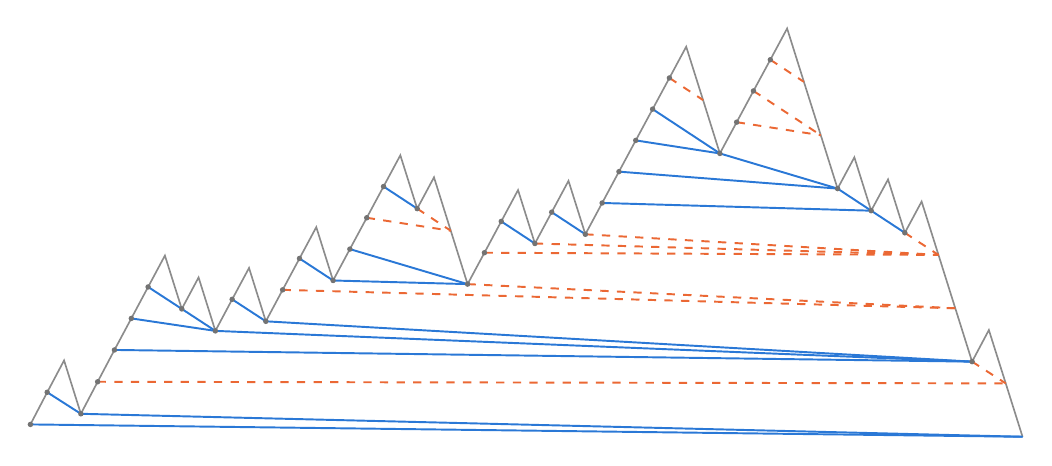
\begin{tikzpicture}[scale=0.9]\dropchordsXXVII\end{tikzpicture}}

\begin{document}
\maketitle

\begin{center}\small
  \copyright\ 2026 Ruud H.G. van Tol. Licensed under \href{https://creativecommons.org/licenses/by/4.0/}{CC BY 4.0}.
\end{center}

\subsection*{How to read this paper}

This paper is an introduction: it shows the rules of the game and leaves the proofs
to the second paper~\cite{Paper2}, where most of them are checked by the proof
assistant Lean~4 (Appendix~\ref{app:lean}). You don't need any of that to follow the
story: you can skip all references to Python and Lean, or look them up in the
appendices. Names in sans-serif, like \lean{admissible\_iff\_chain}, are signposts for
readers who want to look up the proof. Examples can be replayed with the Python script
\texttt{pv.py} (Appendix~\ref{app:pv}); a command looks like \pv{list 4}. At the end
of each chapter, a box lists the key terms. The paper, the Lean proofs and the
scripts were made with Claude (Anthropic) as a working partner;
Appendix~\ref{app:lean} tells how. Appendix~\ref{app:table} lists the first families.

\subsection*{Acknowledgements}

Mike Winkler pointed to the old probability idea behind the parts and checked
the literature. Allan Wechsler read an early draft and suggested how to make it
clearer.

\section{The game}
\label{sec:intro}

\termhere{game}Pick a whole number, say $7$. The \keyterm{game}{game} has two rules:
\begin{center}
\emph{even}: halve it; \quad \emph{odd}: triple it, add one, and halve the result.
\end{center}
(Three times an odd number plus one is always even, so the halving always works.
In the OEIS these rules are A014682\index{OEIS!A014682}~\cite{OEIS_A014682}.)
Play from $7$:
\[
7 \to 11 \to 17 \to 26 \to 13 \to 20 \to 10 \to 5 .
\]
\termhere{drop}After seven steps we are at $5$, below the $7$ we started from. That is where the
game ends: at the \keyterm{drop}{drop}.

The famous version of this game, the Collatz conjecture, does not stop there: it
asks whether every start eventually reaches $1$. Nobody knows. Our game asks
something that looks easier: does every start above $1$ eventually get below
itself? It is not really easier. If every number drops, a start drops to a smaller
number, that one drops to a still smaller number, and so on, and whole numbers
cannot keep getting smaller forever. So the chain of drops ends at $1$. The other way
round, a start above $1$ that reaches $1$ has dropped on the way. Both questions are
the same question (\lean{tDrop\_equiv\_collatzT}), and from here on we never
play past a drop. The start $1$ plays $1 \to 2 \to 1$, and we count that as its
drop.

\subsection*{Families that play alike}

\termhere{family}Play from $5$, $9$ and $13$:
\[
5 \to 8 \to 4, \qquad 9 \to 14 \to 7, \qquad 13 \to 20 \to 10 .
\]
Each is odd, then even, and after two steps it has dropped. The same holds for
every fourth number from $1$ on: $1, 5, 9, 13, 17, \dots$ all play the same two
steps. We call such numbers a \keyterm{family}{family}. Its members land on
$1, 4, 7, 10, 13, \dots$, every third number. Where they go next doesn't matter:
they have dropped already. (How many factors $2$ the numbers after the first step, $2, 8, 14, 20, \dots$,
hold is A375961\index{OEIS!A375961}~\cite{OEIS_A375961}.)

Another family is $3, 19, 35, 51, \dots$, every $16$th number. Its members play
odd, odd, even, even:
\[
3 \to 5 \to 8 \to 4 \to 2, \qquad 19 \to 29 \to 44 \to 22 \to 11,
\]
and land on $2, 11, 20, \dots$, every $9$th number.

The even numbers $2, 4, 6, \dots$ are a family as well: one even step, and they have
dropped.

Here are the first families (Table~\ref{tab:families}).
In the last column, \bw{1} stands for an odd step and \bw{0} for an even one.

\nopagebreak
\begin{herefloat}{table}
\centering
$\begin{array}{l@{\ }r l@{\ }r l}
\toprule
\multicolumn{2}{l}{\text{family}} & \multicolumn{2}{l}{\text{lands on}} & \text{steps} \\
\midrule
2, 4, 6, \dots & \text{(every 2nd)} & 1, 2, 3, \dots & \text{(every number)} & \bw{0} \\
1, 5, 9, \dots & \text{(every 4th)} & 1, 4, 7, \dots & \text{(every 3rd)} & \bw{10} \\
3, 19, \dots & \text{(every 16th)} & 2, 11, \dots & \text{(every 9th)} & \bw{1100} \\
11, 43, \dots & \text{(every 32nd)} & 10, 37, \dots & \text{(every 27th)} & \bw{11010} \\
23, 55, \dots & \text{(every 32nd)} & 20, 47, \dots & \text{(every 27th)} & \bw{11100} \\
7, 135, \dots & \text{(every 128th)} & 5, 86, \dots & \text{(every 81st)} & \bw{1110100} \\
15, 143, \dots & \text{(every 128th)} & 10, 91, \dots & \text{(every 81st)} & \bw{1111000} \\
59, 187, \dots & \text{(every 128th)} & 38, 119, \dots & \text{(every 81st)} & \bw{1101100} \\
\bottomrule
\end{array}$
\caption{The first families, by number of odd steps and lowest member: their members, where they land,
and their steps.}
\label{tab:families}
\end{herefloat}

Two things jump out. First, the gaps $2, 4, 16, 32, 128$ between family members turn
into $1, 3, 9, 27, 81$: powers of two become powers of three. Follow two members side
by side: an even step halves the gap between them, an odd step triples it and
halves it. As long as the gap is still even, the two members are both odd
or both even, and so they play the same steps. Second, the number of steps only
depends on how many of them are odd: $1$ odd step gives $2$ steps, $2$ give $4$,
$3$ give $5$, $4$ give $7$. Now write $3, 9, 27, 81$ in binary: $\bin{11}$, $\bin{1001}$,
$\bin{11011}$, $\bin{1010001}$. They have $2$, $4$, $5$ and $7$ digits.
Chapter~\ref{sec:words} comes back to this.

\nopagebreak
So the game becomes: \emph{does every number above $1$ belong to some family?}
That is still open (Chapter~\ref{sec:open}). On the way we find out:
\begin{itemize}
\item every family spells a word in an alphabet of two letters, and that word alone tells
  which family it is (Chapters~\ref{sec:words} and~\ref{sec:numbers});
\item long words are made of shorter words, and which words fit together depends
  only on how many \bw{1}s they have (Chapter~\ref{sec:chain});
\item that makes the words easy to count (Chapter~\ref{sec:count});
\item there is a faster way to play, and it sorts everything the same way
  (Chapter~\ref{sec:fast}).
\end{itemize}

\subsection*{The sequences in this story}

The On-Line Encyclopedia of Integer Sequences (OEIS) knows many pieces of this
game, each from its own angle. They all get a role here (Table~\ref{tab:oeis}).

\nopagebreak
\begin{herefloat}{table}
\small
\begin{tabular}{@{}c l l@{}}
\toprule
chapter & sequence & in this paper \\
\midrule
\ref{sec:intro} & A014682\index{OEIS!A014682} & the rules of the game \\
\ref{sec:intro} & A375961\index{OEIS!A375961} & factors $2$ in the number after the first step from $1, 5, 9, \dots$ \\
\ref{sec:words} & A000265\index{OEIS!A000265} & the odd part of a word \\
\ref{sec:words} & A020914\index{OEIS!A020914} & the length of the valid words of each Order \\
\ref{sec:words} & A022921\index{OEIS!A022921} & how much that length grows: $1$ or $2$ \\
\ref{sec:words}, \ref{sec:count} & A100982\index{OEIS!A100982} & the number of valid words of each Order \\
\ref{sec:words} & A368514\index{OEIS!A368514} & the numbers in the counting grid \\
\ref{sec:numbers} & A177789\index{OEIS!A177789} & the Collatz-primes of each Order \\
\ref{sec:numbers} & A243115\index{OEIS!A243115} & all Collatz-primes of Order $2$ and up, sorted \\
\ref{sec:numbers} & A122442\index{OEIS!A122442} & the lowest Collatz-prime of each Order \\
\ref{sec:count} & A186008\index{OEIS!A186008} & the Collatz-primes of each Order, as distances \\
\ref{sec:fast} & A375782\index{OEIS!A375782} & slides after a run of 1-stairs \\
\ref{sec:fast} & A324245\index{OEIS!A324245} & the index map of Vaillant and Delarue \\
\ref{sec:fast} & A349414\index{OEIS!A349414} & how much the index changes under that map \\
\ref{sec:fast} & A387325\index{OEIS!A387325} & head and length of the tail of \texttt{1}s swapped \\
\ref{sec:open} & A076227\index{OEIS!A076227} & counts behind the share of numbers not yet in a family \\
\ref{sec:open} & A060412\index{OEIS!A060412} & the lowest floors not yet in a family \\
\bottomrule
\end{tabular}
\caption{The OEIS sequences in this paper, by chapter; the words in the last column are
explained in the chapter named.}
\label{tab:oeis}
\end{herefloat}

\begin{wordbox}
\boxhere{game}the game\index{game@\termlink{game}{game}|textbf} & even: halve; odd: triple, add one, halve. \\
\boxhere{drop}drop\index{drop@\termlink{drop}{drop}|textbf} & the first time the game gets below its start; for $1$,
  the return to $1$. \\
\boxhere{family}family\index{family@\termlink{family}{family}|textbf} & numbers with equal gaps that play the same steps up to
  their drop. \\
A014682\index{OEIS!A014682} & the rules of the game. \\
A375961\index{OEIS!A375961} & factors $2$ in the number after the first step from
  $1, 5, 9, \dots$
\end{wordbox}

%% ======================================================================
\section{Two letters}
\label{sec:words}

Inside a family only the steps matter. So let us look at the steps on their own,
without numbers.

\termhere{letters}The game has an alphabet of just two \keyterm{letters}{letters}, \bw{1} and \bw{0}. \termhere{1step}\termhere{0step}Write \bw{1} for a
\keyterm{1step}{1-step} (odd: triple, add one, halve) and \bw{0} for a \keyterm{0step}{0-step} (even:
halve). \termhere{word}Play a start until it drops, write down its steps, and you get a \keyterm{word}{word}:
$123$ spells \bw{11011010}. As in any language, long words are made of shorter ones,
and a hyphen shows the parts: \bw{1-10-11010}. Chapter~\ref{sec:chain} shows where
the hyphens go. \termhere{order}The number of \bw{1}s in a word is its \keyterm{order}{Order}: \bw{11011010} has
Order $5$.

\termhere{validword}A word that a start spells on its way to its drop is a \keyterm{validword}{valid word}. Which
strings of \bw{1}s and \bw{0}s are valid, and how many are there?

\nopagebreak
Three rules hold for every valid word found so far. \termhere{simplerrule}The second
paper~\cite{Paper2} proves them for the words of a \keyterm{simplerrule}{simpler rule}, the game with its
``add one'' left out and no floor needed. Keep two piles, both starting at $1$: for every
letter double the second pile, and for a \bw{1} also triple the first. The word ends as soon
as the second pile is the bigger one; \bw{10} ends with the piles at $3$ and $4$. Whether
every start spells exactly those words is the second of the two sharper questions of
Chapter~\ref{sec:open}, checked for every Order up to ten million.
\begin{itemize}
\item \emph{A valid word ends with \bw{0}.} A 1-step always goes up, so the drop is
  always a 0-step.
\item \emph{All valid words of the same Order have the same length}: the number of
  binary digits of $3^n$, for Order $n$, as Table~\ref{tab:families}
  suggested. These lengths are $1, 2, 4, 5, 7, 8, 10, \dots$
  (A020914\index{OEIS!A020914}~\cite{OEIS_A020914}), and they grow by $1$ or $2$ at a time
  (A022921\index{OEIS!A022921}~\cite{OEIS_A022921}).
\item \emph{No valid word is the beginning of another one.}
\end{itemize}
The shortest valid word is \bw{0}: start at $2$, halve, done. \termhere{rank}Here are all seven valid
words of Order $5$, sorted as in a dictionary; the position in this list is a
word's \keyterm{rank}{rank}:
\[
\bw{11011010},\; \bw{11011100},\; \bw{11101010},\; \bw{11101100},\; \bw{11110010},\; \bw{11110100},\; \bw{11111000} .
\]

\termhere{oddpart}The \bw{0}s at the end of a valid word add nothing: the Order already fixes
how many letters the word has. Read as a binary number, the word without them is its
\keyterm{oddpart}{odd part} (A000265\index{OEIS!A000265}~\cite{OEIS_A000265}): the number halved as long as it is even.
Distinct valid words have distinct odd parts, and \texttt{pv.py} prints words as odd
parts: \pv{list 5} begins with \texttt{1101101}.

\subsection*{Counting on a grid}

There is a quick way to count valid words without listing them. A word is a walk on
a grid: one step right for every \bw{1}, one step down for every \bw{0}
(Figure~\ref{fig:grid}). Write $1$ at the top left, where every walk starts, and at every
other point the number from the left plus the number from above, taking them from white
circles only. The walk of a valid word ends at a blue circle; why they sit exactly there
is explained in the second paper. The numbers in the blue circles
count the valid words of each Order: $1, 1, 1, 2, 3, 7, 12$ for Orders $0$ to $6$,
and then $30, 85, 173, \dots$ (A100982\index{OEIS!A100982}~\cite{OEIS_A100982}, from Order $1$ on). The
numbers in the white circles, column by column, are A368514\index{OEIS!A368514}~\cite{OEIS_A368514},
which has a $0$ at some of the blue circles. The grid never
needs the words themselves, so it is fast: \pv{count 60} prints the count for
Order $60$, a $25$-digit number, at once.

Such a grid can do more than count. Filled in backwards, from the end of one
Order, it tells at every point in how many ways a valid word of that Order can
still be finished, and with
those numbers the word at any rank can be written down directly. Go letter by
letter: if the rank is at most the number of words that go on with \bw{0}, write
\bw{0}; otherwise write \bw{1} and take that number off the rank. So
\pv{unrank 5 4} gives \bw{11101100}, the fourth word of the list above, and for
Order $60$ the word two thirds of the way down the list comes just as fast, with no
word before it ever listed. \pv{rank} goes the other way.

\nopagebreak
\begin{herefloat}{figure}
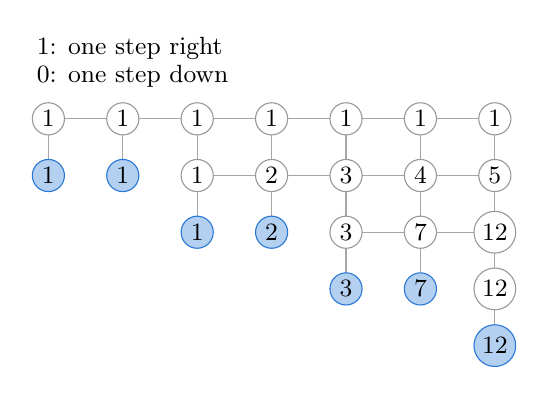
\begin{tikzpicture}[scale=0.9]\countgrid\end{tikzpicture}
\caption{Counting walks. Each circle holds the number in the white circle to its left plus
the number in the white circle above it; a blue circle then holds the number of valid
words of one Order.}
\label{fig:grid}
\end{herefloat}

\begin{wordbox}
\boxhere{letters}letters\index{letters@\termlink{letters}{letters}|textbf} & \bw{1} and \bw{0}, the whole alphabet. \\
\boxhere{1step}\boxhere{0step}1-step, 0-step\index{1-step@\termlink{1step}{1-step}|textbf}\index{0-step@\termlink{0step}{0-step}|textbf} & an odd step (triple, add
  one, halve); an even step (halve). \\
\boxhere{word}word\index{word@\termlink{word}{word}|textbf} & a string of letters; a hyphen shows its parts. \\
\boxhere{order}Order\index{order@\termlink{order}{Order}|textbf} & the number of \bw{1}s in a word. \\
\boxhere{validword}valid word\index{valid word@\termlink{validword}{valid word}|textbf} & the word a start spells up to its drop. \\
\boxhere{rank}rank\index{rank@\termlink{rank}{rank}|textbf} & the position of a word in the dictionary list of its Order. \\
\boxhere{oddpart}odd part\index{odd part@\termlink{oddpart}{odd part}|textbf} & a word without its final \bw{0}s; as a binary number, halved
  while even (A000265\index{OEIS!A000265}). \\
\boxhere{simplerrule}simpler rule\index{simpler rule@\termlink{simplerrule}{simpler rule}|textbf} & two piles from $1$: every letter doubles the second, a \bw{1} also triples
  the first; the word ends when the second is bigger. \\
A020914, A022921\index{OEIS!A020914}\index{OEIS!A022921} & the lengths of valid
  words, and their steps $1$ or $2$. \\
A100982\index{OEIS!A100982} & the number of valid words of each Order. \\
A368514\index{OEIS!A368514} & the numbers in the counting grid.
\end{wordbox}

%% ======================================================================
\section{Every word is a family}
\label{sec:numbers}

\termhere{floor}Time to bring the numbers back, and with them a lift. A number is a \keyterm{floor}{floor},
and the lift only ever stops at whole floors. Board at floor $123$ and play the
game: the lift stops at
\[
185,\ 278,\ 139,\ 209,\ 314,\ 157,\ 236,\ 118 .
\]
Floor $118$ is below $123$, so the ride ends there: the drop of $123$ is $118$. The
buttons pressed on the way, \bw{1} for a 1-step and \bw{0} for a 0-step, spell
\bw{11011010}: a valid word, in parts \bw{1-10-11010}.

Seen from the side, the building has stairs (Figure~\ref{fig:stairs}). Every floor
has exactly one way out: a pole down if it is even, a stair up if it is odd. An even
floor has a hole with a fire pole, numbered \bw{0}: slide
down to half the height, from floor $6$ to floor $3$, from $8$ to $4$, from $4$ to
$2$. An odd floor has a stair numbered \bw{1}, a 1-stair, up: from
floor $3$ to floor $5$, from $7$ to $11$. Stairs and poles run in closed shafts, with a
door only at each end: once you step in, there is no getting off at a floor in
between. Start at floor $3$ and follow stairs and poles:
\bw{1} to floor $5$, \bw{1} to $8$, \bw{0} to $4$, \bw{0} to $2$, below $3$. The labels on the
way spell the word \bw{1100}. The lift takes the same way, only without the
climbing. Any building is too small: in the one of Figure~\ref{fig:stairs}, with $20$ floors,
the stairs from $15$, $17$ and $19$ lead out through the roof. The page \texttt{building.html} that comes with this paper shows the
building on screen: board at any floor and watch the ride to its drop.

\begin{figure}[htbp]
\centering
\begin{tikzpicture}\stairsbuilding\end{tikzpicture}
\caption{A building with $20$ floors, from the side. Left, the stairs numbered \bw{1}
from the odd floors, up; inside, the fire poles numbered \bw{0}, each in a closed
shaft from an even floor down to half its height. The stairs from $15$, $17$ and $19$ lead to floors $23$, $26$ and
$29$, above the roof.}
\label{fig:stairs}
\end{figure}

\subsection*{Families of floors}

Now board at floor $379 = 123 + 256$. The lift stops at
$569, 854, 427, 641, 962, 481, 722$ and $361$: exactly the same buttons, and it
lands on $361 = 118 + 243$. Board at $635 = 123 + 2\cdot 256$ and it lands on
$604 = 118 + 2\cdot 243$. Every $256$th floor from $123$ on plays the same word, and
the whole family lands on every $243$rd floor from $118$ on. Here $256 = 2^8$, one
factor two for each of the $8$ letters, and $243 = 3^5$, one factor three for each of
the $5$ ones: the gaps of Chapter~\ref{sec:intro} again.

Why every $256$th floor? The first button only depends on whether the floor is odd
or even: its last binary digit. The second button depends on the last two binary
digits, the third on the last three, and so on: each letter of the word fixes one more
binary digit of the floor. So a word of $8$ letters picks exactly one floor out of
every $256$. Every word, valid or not, picks such a row of floors; for a valid word
the row is its family
(proved for the words of the simpler rule: \lean{tBits\_classId},
\lean{modEq\_of\_tBits\_eq}, \lean{classEquiv}).

\subsection*{Guess the family}

This also works the other way round: make up a word first, and find its family
afterwards. Start with the shortest word there is: \bw{0}. Which floors play it? A \bw{0}
means ``even, halve'': every even floor plays it, and has dropped after that
one step. So \bw{0} is a valid word, of Order $0$, and it takes care of half of all
floors.

Next, \bw{10}. The first letter asks for an odd floor. Of the odd floors,
$1, 5, 9, \dots$ go to an even floor next and $3, 7, 11, \dots$ to an odd one, so
\bw{10} is the word of every $4$th floor from $1$. They all drop right at the end
($5 \to 8 \to 4$, and $1 \to 2 \to 1$ by our rule), so \bw{10} is valid, of Order $1$:
another quarter. Together with \bw{0}, three quarters of all numbers are done. The word
\bw{1100} adds every $16$th floor from $3$, and so on: each valid word takes its own
share, and no floor plays two words.

Now a longer one, \bw{11010}, of Order $3$. Which floors play it? Find out one letter at a time; each letter doubles the gap, and leaves exactly
two candidates, of which exactly one fits (Table~\ref{tab:guess}).

\begin{table}[htbp]
\centering
\begin{tabular}{@{}l l@{\ }r l l@{}}
\toprule
letters & \multicolumn{2}{l}{candidates} & they play & fits \\
\midrule
\bw{1}     & $1$ or $2$ & (every 2nd) & \bw{1}, \bw{0} & $1$ \\
\bw{11}    & $1$ or $3$ & (every 4th) & \bw{10}, \bw{11} & $3$ \\
\bw{110}   & $3$ or $7$ & (every 8th) & \bw{110}, \bw{111} & $3$ \\
\bw{1101}  & $3$ or $11$ & (every 16th) & \bw{1100}, \bw{1101} & $11$ \\
\bw{11010} & $11$ or $27$ & (every 32nd) & \bw{11010}, \bw{11011} & $11$ \\
\bottomrule
\end{tabular}
\caption{Guessing the family of \bw{11010}, one letter at a time.}
\label{tab:guess}
\end{table}

So \bw{11010} is the word of every $32$nd floor from $11$ on, and $11$ is its
lowest floor. No long ride was needed to find the family: five short ones, each as
long as the letters so far. Is the word valid? Ride from the lowest floor:
$11 \to 17 \to 26 \to 13 \to 20 \to 10$. The first floor below $11$ comes exactly at the
end of the word: valid.

\subsection*{Collatz-primes}

\termhere{collatzprime}The lowest floor of the family of a valid word is its \keyterm{collatzprime}{Collatz-prime} (in
Lean: its \emph{class id}). Like a prime in a sieve, it strikes out its whole family at once;
most Collatz-primes, such as $15$ and $27$, are no prime numbers. Each Order has as many
Collatz-primes as valid words.
Grouped by Order, they are the rows of A177789\index{OEIS!A177789}~\cite{OEIS_A177789}:
\[
2 \;\mid\; 1 \;\mid\; 3 \;\mid\; 11, 23 \;\mid\; 7, 15, 59 \;\mid\;
39, 79, 95, 123, 175, 199, 219 \;\mid\; \dots
\]
Order $0$ is the family of the even floors: one halving, and every even floor has
dropped (A177789 has $0$ where we write $2$). Order $1$ is the family $1, 5, 9, \dots$ of Chapter~\ref{sec:intro}.
Merged and sorted from Order $2$ on, the Collatz-primes are
A243115\index{OEIS!A243115}~\cite{OEIS_A243115}:
$3, 7, 11, 15, 23, 27, 31, 39, 47, 59, \dots$. The lowest one of each Order,
$2, 1, 3, 11, 7, 39, \dots$, is A122442\index{OEIS!A122442}~\cite{OEIS_A122442}
(which has $5$ in the place of the $1$: the lowest floor above $1$).

\nopagebreak
A family can be written down without riding the lift at all: \pv{attrs 1101}
gives Order $3$, Collatz-prime $11$ and drop $10$ for the word \bw{11010} (the final
\bw{0}s are left off). The small ``add one'' of each 1-step decides where exactly the
family lands; the gaps are always powers of two and three (\lean{tStep\_iterate\_shift}).

\begin{wordbox}
\boxhere{floor}floor\index{floor@\termlink{floor}{floor}|textbf} & a number, as seen by the lift: it only stops at
  whole floors. \\
family\index{family@\termlink{family}{family}|textbf} & all floors that play the same valid word; for a word of
  $L$ letters, every $2^L$th floor. \\
\boxhere{collatzprime}Collatz-prime\index{collatz-prime@\termlink{collatzprime}{Collatz-prime}|textbf} & the lowest floor of the family
  of a valid word; in Lean, the class id. \\
A177789, A243115\index{OEIS!A177789}\index{OEIS!A243115} & Collatz-primes by Order;
  all of Order $2$ and up, sorted. \\
A122442\index{OEIS!A122442} & the lowest Collatz-prime of each Order.
\end{wordbox}

%% ======================================================================
\section{Words made of words}
\label{sec:chain}

\termhere{lowestfloor}Where do the hyphens in \bw{1-10-11010} come from? Ride from $123$ again. After the
first step, mark every floor that is lower than all floors before it, counted from
the first step on: $185$, $139$ and $118$. Cut the word there:
\[
\bw{1-10-11010} .
\]
\termhere{part}Each \keyterm{part}{part} after the first \bw{1} is a valid word in its own right: \bw{10} of Order $1$,
\bw{11010} of Order $3$. And for a reason: a part starts at a \keyterm{lowestfloor}{new low} and ends
at the next one, the first floor below where it started: its own drop. Cutting a
walk at its lowest points is an old idea from probability~\cite{Feller1971}, as
M.~Winkler pointed out; what it gives for valid words is new, as far as we know.

\subsection*{Bars and a mountain}

\termhere{subdrop}For every floor on the way, draw a bar to the first later floor below it: its own
drop, a \keyterm{subdrop}{sub-drop} (Figure~\ref{fig:subdrops}). Floor $185$ drops at $139$, and the way there
spells \bw{10}. Floor $139$ drops at $118$, and the way there spells \bw{11010}: the parts
are the bars that run from one new low to the next.

\begin{figure}[htbp]
\centering
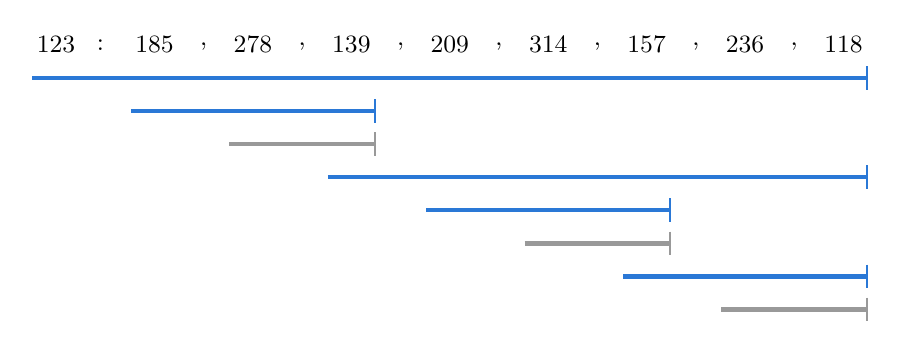
\begin{tikzpicture}\subdropsCXXIII\end{tikzpicture}

\bigskip
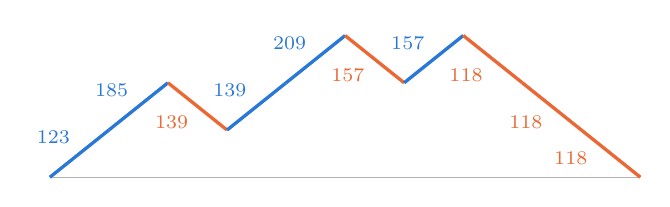
\begin{tikzpicture}\mountainCXXIII\end{tikzpicture}
\caption{Top: the ride of $123$, with a bar from every floor to its own drop; blue
bars start at odd floors, grey ones at even floors. Bottom: the mountain of $123$: one
step up at every odd floor, one step down for each blue bar that ends.}
\label{fig:subdrops}
\end{figure}

\nopagebreak
\termhere{mountain}The blue bars make a \keyterm{mountain}{mountain}. Every odd floor climbs one step; every time the
lift stops below an earlier odd floor for the first time, it comes one step down
for that floor. The mountain of $123$ goes up, up, down, up, up, down, up, down,
down, down: five steps up for the five \bw{1}s, five steps down, and it never goes
below the ground. Every ride that reaches its drop makes such a mountain, because every
bar ends by the drop at the latest. Figure~\ref{fig:chords27} draws the bars of $27$
over its ride.

\emph{The bars belong to the word, not to the start.} Ride from $379$, the next floor
of the family of $123$. The floors are different, $569$, $854$, $427$, \dots, down
to $361$, but every bar starts and ends at the same letters, so the hyphens and the
mountain are the same too. The bars can even be drawn from the word alone, without
riding at all. We checked this for every odd start up to $200\,000$: almost
$600\,000$ bars, each found once by riding and once from the word alone, and they
always agree. The second paper proves it for every ride, on one condition: that the
second of the two sharper questions of Chapter~\ref{sec:open} has the answer yes.

\subsection*{The gluing rule}

\begin{theorem}[Words made of words]
\label{thm:chain}
Every valid word of Order at least $1$ is, in exactly one way, a \bw{1}, followed by
zero or more valid parts of Order at least $1$, followed by nothing or by one extra \bw{0}.
The other way round: glue a \bw{1} and any valid parts together. Whether the result is
a valid word depends only on the Orders of the parts, not on which parts they are.
\end{theorem}
(Proved, as in Chapter~\ref{sec:words}, for the words of the simpler rule:
\lean{exists\_chain}, \lean{chain\_unique}, \lean{admissible\_iff\_chain},
\lean{validOrders\_iff\_dropLast}, \lean{tail\_eq\_zero\_iff}.)

\medskip
\termhere{extra0}The \keyterm{extra0}{extra} \bw{0} is needed when the last part ends just short of the drop. For example
\bw{1100} = \bw{1-10-0}: floor $3$ rides $3 \to 5 \to 8 \to 4 \to 2$. The part \bw{10} is the
ride of $5$ to its drop $4$, but $4$ is not yet below $3$; one more \bw{0} brings it to
$2$. The exact rule for the Orders, and its proof, are in the second paper.

\nopagebreak
Here is the happy accident: \emph{which} parts are used doesn't matter at all, only
their Orders. The seven words of Order $5$ show it (\pv{list 5}, Table~\ref{tab:order5}).

\begin{table}[htbp]
\centering
$\begin{array}{l r l}
\toprule
\text{Orders of the parts} & \text{Collatz-prime} & \text{word} \\
\midrule
1, 3 & 123 & \bw{1-10-11010} \\
1, 3 & 219 & \bw{1-10-11100} \\
3, 1 & 199 & \bw{1-11010-10} \\
3, 1 & 79 & \bw{1-11100-10} \\
4 & 39 & \bw{1-1101100} \\
4 & 175 & \bw{1-1110100} \\
4 & 95 & \bw{1-1111000} \\
\bottomrule
\end{array}$
\caption{The seven valid words of Order $5$, cut into parts, grouped by the Orders of their
parts.}
\label{tab:order5}
\end{table}

Orders $1, 3$: one part of Order $1$ times two of Order $3$, two words. Orders
$3, 1$: two words. Order $4$: all three. The other five ways to split $4$, such as
$2, 2$ or $1, 1, 2$, never appear: a start would drop too early.

\begin{herefloat}{figure}
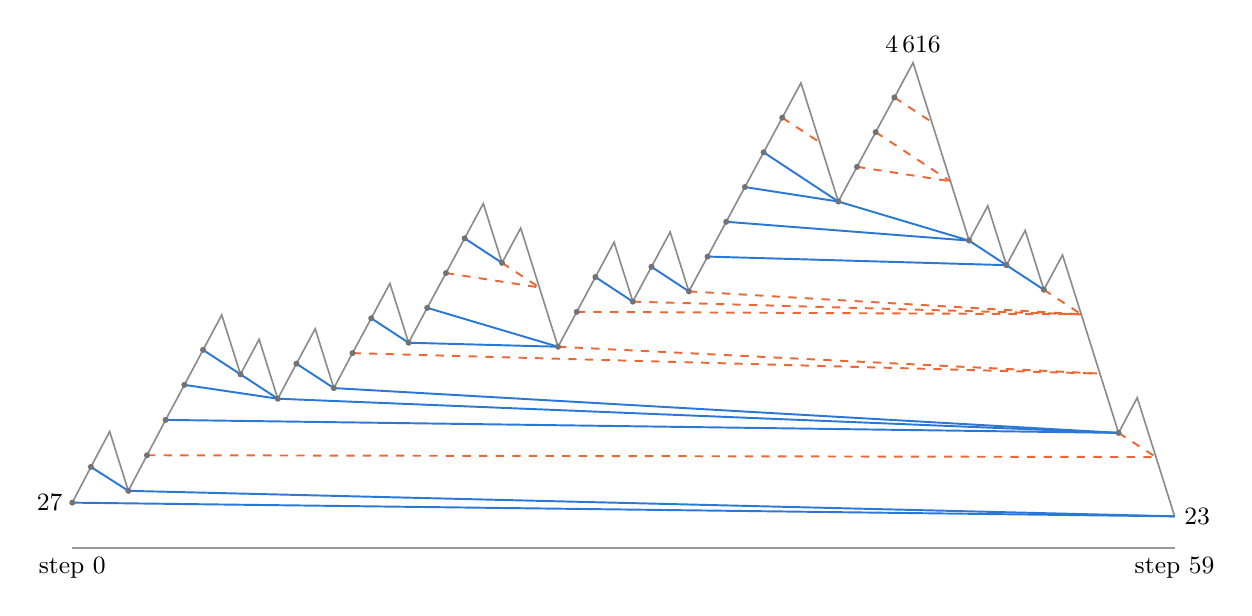
\begin{tikzpicture}\dropchordsXXVII\dropchordsXXVIIlabels\end{tikzpicture}
\caption{The ride of $27$ to its drop at $23$: $59$ steps, up to floor $4\,616$ (the
floors are drawn on a log scale). From every odd floor, a chord to its own drop: solid
when the drop is an odd floor, dashed when it is an even one. These are the blue bars of
Figure~\ref{fig:subdrops}, drawn over the ride; they never cross.}
\label{fig:chords27}
\end{herefloat}

\begin{wordbox}
\boxhere{lowestfloor}new low\index{new low@\termlink{lowestfloor}{new low}|textbf} & a floor lower than all floors before it,
  from the first step on. \\
\boxhere{part}part\index{part@\termlink{part}{part}|textbf} & a piece between two new lows: a valid word of Order
  at least $1$, unless it is the extra \bw{0}. \\
\boxhere{extra0}extra \bw{0}\index{extra 0@\termlink{extra0}{extra \bw{0}}|textbf} & the one \bw{0} that may follow the last part. \\
\boxhere{subdrop}sub-drop\index{sub-drop@\termlink{subdrop}{sub-drop}|textbf} & the drop of a floor on the way; a bar in
  Figure~\ref{fig:subdrops}. \\
\boxhere{mountain}mountain\index{mountain@\termlink{mountain}{mountain}|textbf} & up for every odd floor, down each time the ride first
  gets below that odd floor.
\end{wordbox}

%% ======================================================================
\section{How many words?}
\label{sec:count}

The counting grid of Chapter~\ref{sec:words} gives the number of valid words of each
Order:
\[
1,\ 1,\ 1,\ 2,\ 3,\ 7,\ 12,\ 30,\ 85,\ 173,\ 476,\ 961,\ \dots
\]
for Orders $0, 1, 2, \dots$ (A100982\index{OEIS!A100982}~\cite{OEIS_A100982}, from Order $1$ on). The
gluing rule of Chapter~\ref{sec:chain} gives a second way to find them, and a third
way tells roughly how big they get. As in Chapter~\ref{sec:words}, the proofs count the
words of the simpler rule; the rides spell exactly those words as far as anyone has
checked.

\subsection*{Counting by gluing}

\termhere{gluingcount}A valid word is a \bw{1} followed by parts, and only the Orders of the parts matter. So
list the allowed Orders, multiply the numbers of words for the parts, and add up. For
Order $5$ the parts after the first \bw{1} have Orders adding up to $4$, and the allowed
lists are $1, 3$ and $3, 1$ and $4$:
\[
1 \cdot 2 \;+\; 2 \cdot 1 \;+\; 3 \;=\; 7 .
\]
This \keyterm{gluingcount}{gluing count} works for every Order, with the numbers of all smaller Orders as the only
ingredients (\lean{card\_admSet\_succ}).

\subsection*{About one in $n$}

Take all words of the right length for Order $n$ that start with \bw{1}, valid or not.
For Order $5$: length $8$, a \bw{1} in front, and four more \bw{1}s among the other seven
letters: $35$ words. Exactly $7$ of them are valid, one in five. \termhere{ratcatalan}M.~Winkler~\cite{Winkler2026b} proved that the number of valid words of
Order $n$ is never more than one in $n$ of those words, and exactly one in $n$ at
special Orders like $1, 3, 5, 17, 29, 41$. At those Orders the counts are
\keyterm{ratcatalan}{rational Catalan numbers}, cousins of the Catalan numbers that count mountains
like the one in Figure~\ref{fig:subdrops}.

\subsection*{How often}

\termhere{share}Each valid word takes its own \keyterm{share}{share} of the floors (Chapter~\ref{sec:numbers}): a word
of $L$ letters, one floor in every $2^L$. So the words of one Order together take a
share of $1/2$ for Order $0$, $1/4$ for Order $1$, $1/16$ for Order $2$ and again
$2/32 = 1/16$ for Order $3$, then $3/128$, $7/256$, \dots. These are the shares of
numbers whose drop takes $1, 2, 4, 5, 7, 8, \dots$ steps: the pattern in
A186008\index{OEIS!A186008}~\cite{OEIS_A186008}.

\begin{wordbox}
\boxhere{gluingcount}gluing count\index{gluing count@\termlink{gluingcount}{gluing count}|textbf} & the number of words of an Order, from the
  numbers of words of the smaller Orders. \\
\boxhere{ratcatalan}rational Catalan\index{rational catalan@\termlink{ratcatalan}{rational Catalan}|textbf} & a count of mountains
  under a slanted line; the counts at the special Orders. \\
\boxhere{share}share\index{share@\termlink{share}{share}|textbf} & the part of all floors that a word or an Order
  takes. \\
A100982\index{OEIS!A100982} & the number of valid words of each Order. \\
A186008\index{OEIS!A186008} & the Collatz-primes of each Order, as distances; their shares.
\end{wordbox}

%% ======================================================================
\section{A faster way to play}
\label{sec:fast}

One day a very young engineer visits the building of Chapter~\ref{sec:numbers}. \termhere{longpole}He
counts the holes and poles and has an idea: why slide from $8$ to $4$, then from $4$
to $2$, then from $2$ to $1$, with three holes and three poles, when one \keyterm{longpole}{long pole}
from $8$ straight down to $1$ does the same? \termhere{escalator}And while he is at it, an \keyterm{escalator}{escalator}: from
an odd floor, all the 1-stairs in a row in one go, together with the slide that
follows them. From $27$, which is $\bin{11011}$, the escalator runs
$27 \to 41 \to 62 \to 31$ in one ride.

\termhere{fastride}His building works. The ride of $27$ to its drop takes $59$ steps; the \keyterm{fastride}{fast
ride}, with escalators and long poles, takes $20$:
\begin{gather*}
27,\ 31,\ 121,\ 91,\ 103,\ 175,\ 445,\ 334,\ 167,\ 283,\ 319,\\
1822,\ 911,\ 2308,\ 577,\ 433,\ 325,\ 244,\ 61,\ 46,\ 23 .
\end{gather*}
It climbs the same number of 1-stairs, so the Order stays the same (\lean{order\_preservation}).

\subsection*{The accident}

\begin{figure}[p]
\centering
\begin{tikzpicture}\comicengineer\end{tikzpicture}
\caption{The young engineer and his long pole, all the way down to $1$, as the famous
version does.}
\label{fig:comic}
\end{figure}


But the engineer forgot that the game ends at the drop (Figure~\ref{fig:comic}). Board at
floor $3$: up the stairs to $8$ ($3 \to 5 \to 8$), and the long pole from $8$ goes
straight down to $1$, right past floor $2$, where your game should have ended. \termhere{freelunch}In the
game, the first floor below your start is a \keyterm{freelunch}{free lunch}: everything after it is the
game of a smaller start, which plays it on its own (Chapter~\ref{sec:intro}). Sliding on
wins nothing, and loses the one place where you were supposed to get off. So the fast
ride has to remember where the drop was: on the last pole, you may have to get off
halfway.

\subsection*{A trick in binary}

The escalator is a small trick on the binary digits of the floor. Take $91 = \bin{1011011}$,
a floor of the fast ride of $27$. Cut off its last \texttt{0} and the \texttt{1}s after it (put a
\texttt{0} in front if there is none): \texttt{011}, two \texttt{1}s. Multiply what is left,
$\bin{1011} = 11$, by $3$ for each cut \texttt{1}: $11 \cdot 9 = 99$. Add $1$ for one cut
\texttt{1}, $4$ for two, $13$ for three (that is \texttt{1}, \texttt{11}, \texttt{111} in base
$3$): $99 + 4 = 103$, the next floor of that fast ride. How many slides follow a run of 1-stairs is
A375782\index{OEIS!A375782}~\cite{OEIS_A375782}. Vaillant and Delarue's related map~\cite{VaillantDelarue2019}
works on the index $n$ of the odd floor $2n+1$
(A324245\index{OEIS!A324245}~\cite{OEIS_A324245}); how much that index changes is
A349414\index{OEIS!A349414}~\cite{OEIS_A349414}. And just for fun: the same cut, at the
last \texttt{0}, splits a number into a head and a tail of \texttt{1}s, and swapping the head with the length of the tail gives
A387325\index{OEIS!A387325}~\cite{OEIS_A387325}.

\subsection*{Everything sorts alike}

Write the fast ride of each Collatz-prime as a list: how many 1-stairs each escalator
climbs, and how long each pole is, with a minus sign for a pole. Sort the Collatz-primes
of one Order by their words, as in a dictionary, or by these lists, number by number: they
come out sorted the same way
(\lean{tBits\_lt\_iff\_markedVector\_lt}, for Collatz-primes that drop at the end of
their word). The families can even be grown sorted this way
directly, like a tree where every word sprouts its possible next pieces
(\lean{lex\_enumeration}); the rank of Chapter~\ref{sec:words} is the place in this
sorting.

\begin{wordbox}
\boxhere{escalator}escalator\index{escalator@\termlink{escalator}{escalator}|textbf} & all 1-stairs in a row at once, with the slide after
  them. \\
\boxhere{longpole}long pole\index{long pole@\termlink{longpole}{long pole}|textbf} & all slides in a row at once, down to an odd
  floor. \\
\boxhere{fastride}fast ride\index{fast ride@\termlink{fastride}{fast ride}|textbf} & the ride by escalators and long poles; it may pass
  the drop on its last pole. \\
\boxhere{freelunch}free lunch\index{free lunch@\termlink{freelunch}{free lunch}|textbf} & the drop: everything after it is the game of a
  smaller start. \\
A375782, A349414\index{OEIS!A375782}\index{OEIS!A349414} & slides after a run of 1-stairs;
  the index change under Vaillant and Delarue's map. \\
A324245\index{OEIS!A324245} & the index map of Vaillant and Delarue. \\
A387325\index{OEIS!A387325} & head and length of the tail of \texttt{1}s swapped.
\end{wordbox}

%% ======================================================================
\section{What nobody knows yet}
\label{sec:open}

\termhere{bigquestion}Here the game gets hard, for everybody. The \keyterm{bigquestion}{big question} is short: \emph{does every
floor above $1$ drop?} Put in the words of this paper: does every floor above $1$
belong to the family of some valid word? If the answer is yes, then by
Chapter~\ref{sec:intro} the famous version is settled too. Nobody knows. The second
paper splits the question into two sharper ones and shows what each would give.
First: does every floor above $1$ sooner or later spell a word of the simpler rule of
Chapter~\ref{sec:words}? Second: does its ride then really drop at the end of that
word, and not later?

\subsection*{What we do know}

\begin{itemize}
\item Every floor up to $984\,572\,779\,224$, almost $10^{12}$, drops: our own computer
  check, made for the second paper, went through them all. The closest call we know is
  $47$: of the floors up to twenty million, it comes nearest to riding on past the end of its word,
  in a sense the second paper makes exact. Its word has Order $34$, and its ride ends
  on floor $46$.
\item The share of numbers not yet in any family of Order at most $n$ shrinks:
  $1/2$, $1/4$, $3/16$, $1/8$, $13/128$, $19/256$, $1/16$, \dots{} for $n = 0, 1, 2, \dots$
  (A076227\index{OEIS!A076227}~\cite{OEIS_A076227}, divided by powers of two).
  Almost every number drops: R.~Terras proved that in 1976~\cite{Terras1976}.
\item The lowest floor above $1$ not yet in a family changes only now and then:
  $2$ before any family, then $3$, $7$, $27$, $703$, $10087$, $35655$, \dots
  (A060412\index{OEIS!A060412}~\cite{OEIS_A060412}).
\end{itemize}

\subsection*{Loops}

\termhere{loop}Could a ride run in a \keyterm{loop}{loop}? The ride $1 \to 2 \to 1$ does: it is the drop of $1$. Any other loop would have a lowest floor, and that floor would never drop.
So if every floor above $1$ drops, there is no other loop. None is known.

\subsection*{Two kinds of question}

Which family a floor belongs to depends only on its last binary digits
(Chapter~\ref{sec:numbers}): a question about digits, blind to size. Whether a floor
drops at the end of that word depends on its size as well: a large floor does, and only
for the smallest floors of a family can the ``add one''s make the ride go on (the second
sharper question). The big question sits exactly where these two worlds
meet, and that is what makes it so hard~\cite{Lagarias1985}.

\begin{wordbox}
\boxhere{bigquestion}the big question\index{big question@\termlink{bigquestion}{big question}|textbf} & does every floor above $1$ drop? \\
\boxhere{loop}loop\index{loop@\termlink{loop}{loop}|textbf} & a ride that comes back to its start; only $1 \to 2 \to 1$ is
  known. \\
A076227\index{OEIS!A076227} & counts behind the share of numbers not yet in a
  family. \\
A060412\index{OEIS!A060412} & the lowest floors not yet in a family.
\end{wordbox}

%% ======================================================================
\appendix

\section{pv.py}
\label{app:pv}

\texttt{pv.py} is a small Python script (Python~3.8 or later, no extra packages)
that knows every valid word of every Order, without storing any lists. A word is
typed as its \emph{key}: the word without its final \bw{0}s, so \bw{1101} stands for
\bw{11010}. Table~\ref{tab:pv} lists the commands.

\begin{table}[htbp]
\centering
\begin{tabular}{@{}ll@{}}
\toprule
command & result \\
\midrule
\texttt{attrs KEY \dots} & length, Order, Collatz-prime, drop, rank, parts \\
\texttt{count O \dots} & the number of valid words of Order $O$
  (A100982\index{OEIS!A100982}) \\
\texttt{list O [N]} & the valid words of Order $O$: the first $N$ ($50$ without $N$) \\
\texttt{rank KEY} / \texttt{unrank O R} & rank of a word / word of a rank \\
\texttt{test} & the self-test \\
\bottomrule
\end{tabular}
\caption{The commands of \texttt{pv.py}.}
\label{tab:pv}
\end{table}

A short session:
\begin{lstlisting}
$ ./pv.py attrs 1101
Attrs(key='1101', p2=5, p3=3, x=11, drop=10, rank=1, rho=23,
      chain=['1', '1'], code=[(1, 1), (1, 1)])
$ ./pv.py count 5 20
5 7
20 5936673
\end{lstlisting}
Here \texttt{p2} is the length, \texttt{p3} the Order, \texttt{x} the Collatz-prime
and \texttt{drop} where it lands, \texttt{rank} its rank, \texttt{rho} a number for the
second paper; \texttt{chain} lists the keys of the parts, and
\texttt{code} each part as (Order, rank). The script has more commands, for the second
paper.

\section{The Lean formalization}
\label{app:lean}

The Lean~4 project \lean{AcceleratedCollatz} (with Mathlib) proves the results that the
second paper cites by a Lean name, without gaps (what is still open enters as a condition); the sans-serif names in this paper point there. A
self-contained file \texttt{ChainDecomposition.lean} holds the parts, the gluing rule
and the counts, with Mathlib as its only dependency.

\subsection*{How this was made}

The Lean files, the scripts and this text were written in conversation with
Claude (Anthropic): ideas were tried numerically first, then stated and proved in
Lean, compiled locally, and every open end was logged for the next session. Some
of it went better than planned. Once the words were cut at their lowest points, the
parts turned out to be valid words again, glued by a rule on their Orders only; the
proofs of Chapters~\ref{sec:chain} and~\ref{sec:count} then became short and clean. An
independent audit, commissioned by M.~Winkler, compiled an earlier version of
\texttt{ChainDecomposition.lean} and checked its proofs once more with a second checker. The
same workflow is open to any reader: the Lean proofs can be checked on any computer,
and \texttt{pv.py} replays the examples. Table~\ref{tab:lean} lists the main lean-files.

\begin{table}[htbp]
\centering
\begin{tabular}{@{}>{\raggedright\arraybackslash}p{0.42\linewidth}>{\raggedright\arraybackslash}p{0.5\linewidth}@{}}
\toprule
lean-file & content \\
\midrule
\lean{DropEquivalenceT} & the drop game and the famous version are the same question \\
\lean{AdmissibleLength} & valid words: length and beginnings \\
\lean{TCorrespondence}, \lean{TAffine} & every word is a family; where it lands \\
\lean{TChain$\{$,Orders$\}$} & words made of words, the gluing rule \\
\lean{TCount}, \lean{TBinomial} & how many words \\
\lean{RMap}, \lean{OrderPreservation} & the fast ride \\
\lean{TLex}, \lean{TVectorLex} & everything sorts alike \\
\bottomrule
\end{tabular}
\caption{The main lean-files; braces group names as in a shell, so \lean{TChain$\{$,Orders$\}$} is \lean{TChain} and \lean{TChainOrders}.}
\label{tab:lean}
\end{table}

\noindent The full list of lean-files is in the second paper.

\section{The first families}
\label{app:table}

Every family of Order $6$ or less, and the first of Order $7$, by rank: its
floors (the Collatz-prime plus $i\cdot 2^L$, for $i = 0, 1, 2, \dots$), where they land, the fast ride
of the Collatz-prime (Chapter~\ref{sec:fast}), and the share of all floors
not yet in any family listed so far (Table~\ref{tab:first}).

\begin{table}[htbp]
\centering
\small
\begin{tabular}{@{}r r@{\,+\,$i\cdot$}l @{\,$\to$\,} r@{\,+\,$i\cdot$}l l r@{}}
\toprule
Order & \multicolumn{4}{c}{family $\to$ lands on} & fast ride & left \\
\midrule
0 &   2 & $2^1$    &   1 & $3^0$  & $(2, 1)$                    & $1/2$ \\
1 &   1 & $2^2$    &   1 & $3^1$  & $(1, 1)$                    & $1/4$ \\
2 &   3 & $2^4$    &   2 & $3^2$  & $(3, 4, 2)$                 & $3/16$ \\
3 &  11 & $2^5$    &  10 & $3^3$  & $(11, 13, 10)$              & $5/32$ \\
3 &  23 & $2^5$    &  20 & $3^3$  & $(23, 40, 20)$              & $1/8$ \\
4 &  59 & $2^7$    &  38 & $3^4$  & $(59, 67, 76, 38)$          & $15/128$ \\
4 &   7 & $2^7$    &   5 & $3^4$  & $(7, 13, 10, 5)$            & $7/64$ \\
4 &  15 & $2^7$    &  10 & $3^4$  & $(15, 40, 10)$              & $13/128$ \\
5 & 123 & $2^8$    & 118 & $3^5$  & $(123, 139, 157, 118)$      & $25/256$ \\
5 & 219 & $2^8$    & 209 & $3^5$  & $(219, 247, 418, 209)$      & $3/32$ \\
5 & 199 & $2^8$    & 190 & $3^5$  & $(199, 337, 253, 190)$      & $23/256$ \\
5 &  39 & $2^8$    &  38 & $3^5$  & $(39, 67, 76, 38)$          & $11/128$ \\
5 &  79 & $2^8$    &  76 & $3^5$  & $(79, 202, 101, 76)$        & $21/256$ \\
5 & 175 & $2^8$    & 167 & $3^5$  & $(175, 445, 334, 167)$      & $5/64$ \\
5 &  95 & $2^8$    &  91 & $3^5$  & $(95, 364, 91)$             & $19/256$ \\
6 &  507 & $2^{10}$ &  362 & $3^6$  & $(507, 571, 643, 724, 362)$ & $75/1024$ \\
6 &  347 & $2^{10}$ &  248 & $3^6$  & $(347, 391, 661, 496, 248)$ & $37/512$ \\
6 &  923 & $2^{10}$ &  658 & $3^6$  & $(923, 1039, 2632, 658)$ & $73/1024$ \\
6 &  583 & $2^{10}$ &  416 & $3^6$  & $(583, 985, 739, 832, 416)$ & $9/128$ \\
6 &  423 & $2^{10}$ &  302 & $3^6$  & $(423, 715, 805, 604, 302)$ & $71/1024$ \\
6 &  999 & $2^{10}$ &  712 & $3^6$  & $(999, 1687, 2848, 712)$ & $35/512$ \\
6 &  975 & $2^{10}$ &  695 & $3^6$  & $(975, 2470, 1235, 1390, 695)$ & $69/1024$ \\
6 &  815 & $2^{10}$ &  581 & $3^6$  & $(815, 2065, 1549, 1162, 581)$ & $17/256$ \\
6 &  367 & $2^{10}$ &  262 & $3^6$  & $(367, 931, 1048, 262)$ & $67/1024$ \\
6 &  735 & $2^{10}$ &  524 & $3^6$  & $(735, 2794, 1397, 1048, 524)$ & $33/512$ \\
6 &  287 & $2^{10}$ &  205 & $3^6$  & $(287, 1093, 820, 205)$ & $65/1024$ \\
6 &  575 & $2^{10}$ &  410 & $3^6$  & $(575, 3280, 410)$ & $1/16$ \\
7 & 1019 & $2^{12}$ &  545 & $3^7$  & $(1019, 1147, 1291, 1453, 1090, 545)$ & $255/4096$ \\
\bottomrule
\end{tabular}
\caption{The first families.}
\label{tab:first}
\end{table}
Each fast ride ends at the drop: where its last piece is a pole, you may have to get
off halfway, as in $(3, 4, 2)$.

\begin{thebibliography}{99}
\bibitem{Feller1971} W.~Feller, \emph{An Introduction to Probability Theory and
  Its Applications}, Vol.~II, 2nd ed., Wiley, 1971, Chapter~XII.
\bibitem{Lagarias1985} J.~C. Lagarias, \emph{The $3x+1$ problem and its
  generalizations}, Amer.\ Math.\ Monthly \textbf{92} (1985), 3--23.
\bibitem{OEIS_A000265} OEIS Foundation Inc., \emph{Sequence A000265},
  \url{https://oeis.org/A000265}.
\bibitem{OEIS_A014682} OEIS Foundation Inc., \emph{Sequence A014682},
  \url{https://oeis.org/A014682}.
\bibitem{OEIS_A020914} OEIS Foundation Inc., \emph{Sequence A020914},
  \url{https://oeis.org/A020914}.
\bibitem{OEIS_A022921} OEIS Foundation Inc., \emph{Sequence A022921},
  \url{https://oeis.org/A022921}.
\bibitem{OEIS_A060412} OEIS Foundation Inc., \emph{Sequence A060412},
  \url{https://oeis.org/A060412}.
\bibitem{OEIS_A076227} OEIS Foundation Inc., \emph{Sequence A076227},
  \url{https://oeis.org/A076227}.
\bibitem{OEIS_A100982} OEIS Foundation Inc., \emph{Sequence A100982},
  \url{https://oeis.org/A100982}.
\bibitem{OEIS_A122442} OEIS Foundation Inc., \emph{Sequence A122442},
  \url{https://oeis.org/A122442}.
\bibitem{OEIS_A177789} OEIS Foundation Inc., \emph{Sequence A177789},
  \url{https://oeis.org/A177789}.
\bibitem{OEIS_A186008} OEIS Foundation Inc., \emph{Sequence A186008},
  \url{https://oeis.org/A186008}.
\bibitem{OEIS_A243115} OEIS Foundation Inc., \emph{Sequence A243115},
  \url{https://oeis.org/A243115}.
\bibitem{OEIS_A324245} OEIS Foundation Inc., \emph{Sequence A324245},
  \url{https://oeis.org/A324245}.
\bibitem{OEIS_A349414} OEIS Foundation Inc., \emph{Sequence A349414},
  \url{https://oeis.org/A349414}.
\bibitem{OEIS_A368514} OEIS Foundation Inc., \emph{Sequence A368514},
  \url{https://oeis.org/A368514}.
\bibitem{OEIS_A375782} OEIS Foundation Inc., \emph{Sequence A375782},
  \url{https://oeis.org/A375782}.
\bibitem{OEIS_A375961} OEIS Foundation Inc., \emph{Sequence A375961},
  \url{https://oeis.org/A375961}.
\bibitem{OEIS_A387325} OEIS Foundation Inc., \emph{Sequence A387325},
  \url{https://oeis.org/A387325}.
\bibitem{Terras1976} R.~Terras, \emph{A stopping time problem on the positive
  integers}, Acta Arith.\ \textbf{30} (1976), 241--252.
\bibitem{VaillantDelarue2019} N.~Vaillant and P.~Delarue, \emph{The hidden face of the
  $3x+1$ problem. Part I: Intrinsic algorithm} (2019); linked from OEIS A324245.
\bibitem{Paper2} Ruud H.G. van Tol and Mike Winkler, \emph{Collatz, but stop at the drop; A game with two
  letters: the proofs} (2026).
\bibitem{Winkler2026b} M.~Winkler, \emph{Admissible $qx+1$ sequences,
  semiconvergents, and rational Catalan numbers}, arXiv:2609.22303 (2026).
\end{thebibliography}

\printindex

\end{document}
